%; whizzy paragraph
%; whizzy-paragraph "^\\\\dancersection"
% -initex iniptex -latex platex -format platex -bibtex jbibtex -fmt fmt
% 以上 whizzytex を使用する場合の設定。

%     Tokyo Debian Meeting resources
%     Kansai Debian Meeting resources
%     Copyright (C) 2008 Junichi Uekawa
%     Copyright (C) 2008 Nobuhiro Iwamatsu

%     This program is free software; you can redistribute it and/or modify
%     it under the terms of the GNU General Public License as published by
%     the Free Software Foundation; either version 2 of the License, or
%     (at your option) any later version.

%     This program is distributed in the hope that it will be useful,
%     but WITHOUT ANY WARRANTY; without even the implied warranty of
%     MERCHANTABILITY or FITNESS FOR A PARTICULAR PURPOSE.  See the
%     GNU General Public License for more details.

%     You should have received a copy of the GNU General Public License
%     along with this program; if not, write to the Free Software
%     Foundation, Inc., 51 Franklin St, Fifth Floor, Boston, MA  02110-1301 USA

%   Pdf作成手順
% dvipdfmx debianmeetingresume2011-fuyu.dvi
%  preview (shell-command (concat "evince " (replace-regexp-in-string "tex$" "pdf"(buffer-file-name)) "&"))
% 画像ファイルを処理するためにはebbを利用してboundingboxを作成。
%(shell-command "cd image2012-fuyu; ebb *.png")


% progress memo:
% 2014/6-2014/11がマージ対象
% イベント等でない場合は理由を書くこと。
% 必要な変更点は FIXME で記録しています。

%%ここからヘッダ開始。

\documentclass[mingoth,a4paper]{jsarticle}
\usepackage{monthlyreport}
\usepackage[dvips]{xy} % for advi workaround. Bug #452044
\usepackage{iwamatsu}
\usepackage{ulem}

% tikz picture の為のマクロ設定 for 201407 tokyo
\usepackage[dvipdfmx]{graphicx}
\usepackage{tikz}

% ページ調整のため部分的に2段組に
\usepackage{multicol}

\begin{document}

\begin{titlepage}
\thispagestyle{empty}

\hspace*{-2.5cm}

\includegraphics{image2012-natsu/gudeb.eps}\\
\\
\\
\rotatebox{10}{\fontsize{32}{32} {\gt 東京エリア/関西Debian勉強会}}

%\vspace*{-1.5cm}
\hspace*{11cm}
\includegraphics[height=6cm]{image200502/openlogo-nd.eps}\\
\vspace*{0.1cm}
\hfill あんどきゅめんてっど でびあん 2014年冬号 2014年12月30日 初版発行
\end{titlepage}

\newpage
\thispagestyle{empty}\mbox{}
\newpage

% section の代わりの環境 -- 改訂する。
\renewcommand{\dancersection}[2]{%
\newpage
あんどきゅめんてっど でびあん 2014年冬号
%
% top line
\vspace{0.1mm}\\
{\color{dancerlightblue}\rule{\hsize}{2mm}}

%
% middle text
%
\begin{minipage}[t]{0.6\hsize}
\color{dancerdarkblue}
\vspace{1cm}
\section{#1}
\hfill{}#2\\
\end{minipage}
\begin{minipage}[t]{0.4\hsize}
\vspace{-2cm}
\hfill{}
\includegraphics[height=8cm]{image200502/openlogo-nd.eps}\\
\vspace{-5cm}
\end{minipage}
%
%
{\color{dancerdarkblue}\rule{0.74\hsize}{2mm}}
%
\vspace{2cm}
}

\setcounter{page}{1}
\begin{minipage}[]{0.2\hsize}
 \definecolor{titleback}{gray}{0.9}
 \colorbox{dancerlightblue}{\rotatebox{90}{\fontsize{80}{80}
{\gt \color{dancerdarkblue}デビアン勉強会} }}
\end{minipage}
\begin{minipage}[]{0.8\hsize}
\hrule
\vspace{1mm}
\hrule
\setcounter{tocdepth}{1}
{\small
 \tableofcontents}
\vspace{1mm}
\hrule
\vspace{3cm}

\end{minipage}

% FIXME: 本文を追加すること。
%-------------------------------------------------------------------------------
\dancersection{Introduction}{DebianJP}
%-------------------------------------------------------------------------------

\subsection{東京エリアDebian勉強会}

 Debian勉強会へようこそ。これからDebianの世界にあしを踏み入れると
 いう方も、すでにどっぷりとつかっているという方も、月に一回Debianについ
 て語りませんか?

 Debian勉強会の目的は下記です。

\begin{itemize}
 \item \underline{Debian Developer} (開発者)の育成。
 \item 日本語での ``\underline{開発に関する情報}'' を整理してまとめ、アップデートする。
 \item \underline{場}の提供。
 \begin{itemize}
  \item 普段ばらばらな場所にいる人々が face-to-face で出会える場を提供
    する。
  \item Debian のためになることを語る場を提供する。
  \item Debianについて語る場を提供する。
 \end{itemize}
\end{itemize}

 Debianの勉強会ということで究極的には参加者全員がDebian Packageをがりがり
 と作るスーパーハッカーになった姿を妄想しています。情報の共有・活用を通し
 て Debianの今後の能動的な展開への土台として、 ``場'' としての空間を提供す
 るのが目的です。

\subsection{関西 Debian 勉強会}

 関西 Debian 勉強会はDebian GNU/Linux のさまざ
 まなトピック(新しいパッケージ、Debian 特有の機能の仕組、Debian 界隈で起
 こった出来事、などなど)について話し合う会です。

 目的として次の三つを考えています。
 \begin{itemize}
  \item MLや掲示板ではなく、直接顔を合わせる事での情報交換の促進
  \item 定期的に集まれる場所
  \item 資料の作成
 \end{itemize}

 それでは、楽しい一時をお楽しみ下さい。

%201410 OSC tokyo
%-------------------------------------------------------------------------------
\dancersection{Debian Updates}{岩松 信洋}
%-------------------------------------------------------------------------------
\subsection{ポイントリリース}

\begin{itemize}
\item Debian 7 更新状況 (Wheezy)
\begin{itemize}
\item 2014-04-26 Debian 7 更新: 7.5 リリース
\item 2014-07-12 Debian 7 更新: 7.6 リリース
\end{itemize}
\item Debian 6 更新状況 (Squeeze)
\begin{itemize}
\item 2014-07-19 Debian 6.0 更新: 6.0.10 リリース
\end{itemize}
\end{itemize}

\begin{center}
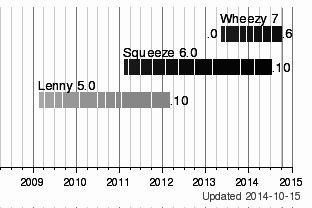
\includegraphics[scale=0.7]{image201410/debian-release-201410-cut_mono.png}
\end{center}



\subsection[containsverbatim]{Long Term Support 開始}
\begin{itemize}
\item 2014/5/31 に Debian 6.x サポート終了
\item 2014/5/27 Debian 6.x 長期サポート (Long Term Support、LTS)開始
\begin{itemize}
\item Debian GNU/Linux 6.x
向けのセキュリティ更新を2016年2月6日まで提供(Squeezeのリリースから5年)
\item i386 と amd64 だけをサポート
\item 全てのパッケージがサポートされるわけではなく、サポート対象から外されるものもある
\item サポート対象外のパッケージはdebian-security-supportパッケージで管理されている
(check-support-status コマンドで確認できる)
\end{itemize}
\end{itemize}

\begin{commandline}
deb http://http.debian.net/debian/ squeeze main

deb http://http.debian.net/debian squeeze-lts main
\end{commandline}



\subsection{tracker.debian.org}
\begin{itemize}
\item Debian Package Tracking System(\url{packages.qa.debian.org})の置き換え
\item Django framework を使用
\end{itemize}

\begin{center}
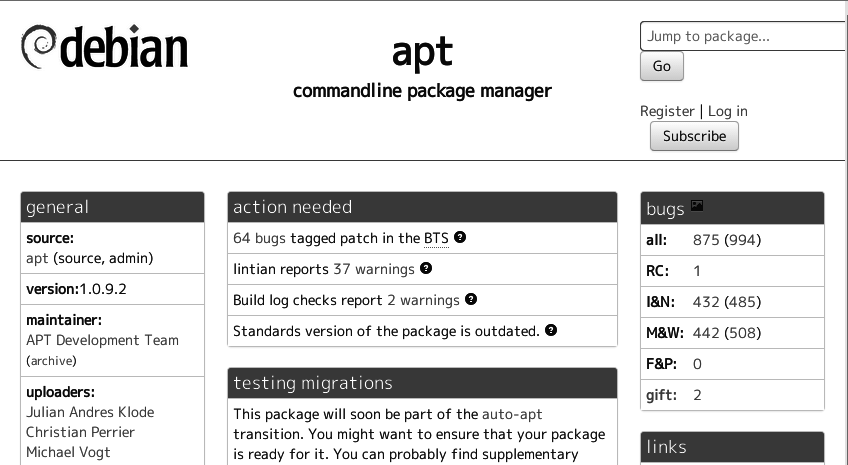
\includegraphics[scale=0.3]{image201410/tracker_mono.png}
\end{center}




\subsection{Debconf 14}

\begin{center}

\includegraphics[scale=0.25]{image201410/debconf14-logo_mono.png}
\end{center}

\begin{itemize}
\item 8月23日から31日まで、アメリカのポートランドで開催
\item 参加者は約300名(日本からの参加は2名)
\item カンファレンスのビデオや資料は \url{http://debconf14.debconf.org}
から参照可能
\item Debconf15 は ドイツのハイデルベルクで開催
\end{itemize}


\subsection{Debian 8.0 状況}

近日フリーズ

\begin{minipage}{0.55\hsize}
\begin{itemize}
\item 11/5 にフリーズ(予定)
\item フリーズ: パッケージの新しいバージョンへの更新を停止
\begin{itemize}
\item 9/5 にABI更新をフリーズ
\item 10/5 から testing へのマイグレーションを5日から10日に切り替え
\end{itemize}
\end{itemize}
\end{minipage}
\begin{minipage}{0.39\hsize}
\begin{center}
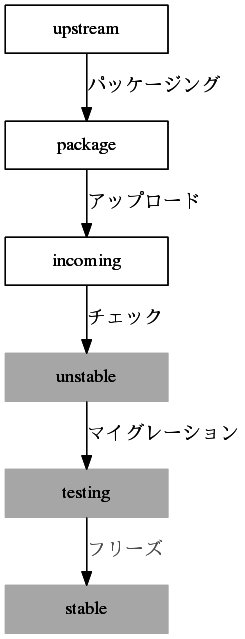
\includegraphics[scale=0.3]{image201410/lifesycle-package_mono.png}
\end{center}
\end{minipage}


\subsection{リリースゴール}
\begin{itemize}
\item systemd
\item piuparts
\item SELinux
\item CrossToolchains
\item CrossBuildableBase
\item utf-8
\item debian/rules honor CC and CXX
\item Clang as secondary compiler
\item Security hardening build flags
\end{itemize}



\subsection{リリースゴールからはずされたもの}
\begin{itemize}
\item pkg-php-tools 移行(PEAR:PHP Extension and Application Repositoryサポート)
\end{itemize}


\subsection{サポートアーキテクチャ}

\begin{itemize}
\item IN: 未定
  \begin{itemize}
  \item arm64, ppcel64 はまだ決定ではない。11月1日の状況によって決まる
  %\item \url{https://lists.debian.org/debian-devel-announce/2014/09/msg00002.html}
  \item x32 は入らなかった模様。
  \end{itemize}
\item OUT: ia64、sparc、s390
\begin{itemize}
\item ia64 はdebian-ports でメンテナンス
\item s390 は s390x に移行
\end{itemize}
\end{itemize}



\subsection{デフォルト init システム}

\begin{itemize}
\item Linux のデフォルトの init システムが systemd に
\item minimal でインストールしても /sbin/init が systemd
\end{itemize}



\subsection{デフォルト Desktop Environment}

\begin{itemize}
\item GNOME
\item 他のDEが tasksel で選択可能に
\begin{center}
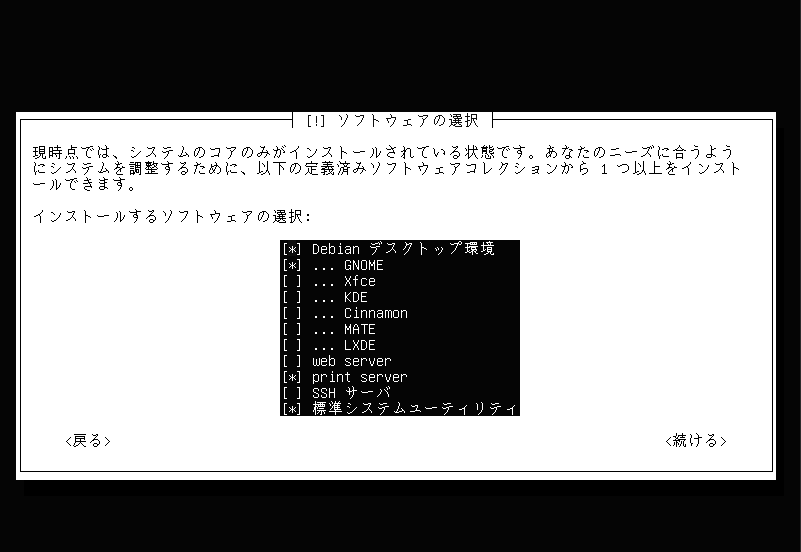
\includegraphics[scale=0.3]{image201410/instaler-tasksel_mono.png}
\end{center}

\end{itemize}


\subsection{auto-removal によるリリース対策}
\begin{itemize}
\item RCバグに14日なにも進展がない場合、そのバグ
をもつパッケージは自動的にtestingから削除される。
\end{itemize}


\subsection{auto-removal によるリリース対策}
\begin{center}
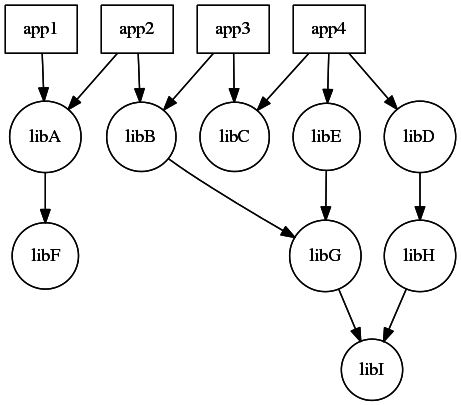
\includegraphics[scale=0.4]{image201410/auto-rm_mono.png}
\end{center}


\subsection{auto-removal によるリリース対策}
\begin{center}
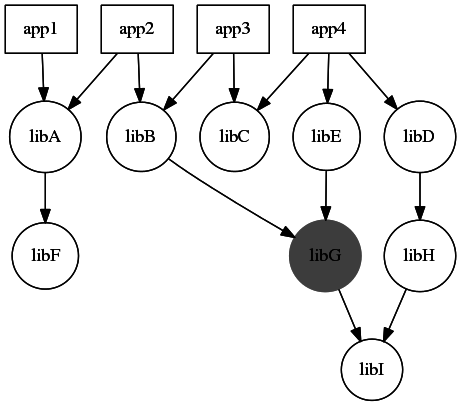
\includegraphics[scale=0.4]{image201410/auto-rm2_mono.png}

libG が auto-rm される
\end{center}


\subsection{auto-removal によるリリース対策}
\begin{center}
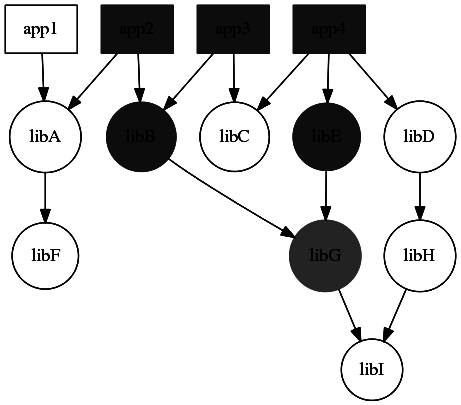
\includegraphics[scale=0.4]{image201410/auto-rm3_mono.png}

libG に依存しているパッケージも auto-rm される
\end{center}


\subsection{auto-removal によるリリース対策}
\begin{itemize}
\item RCバグに14日なにも進展がない場合、そのバグ
をもつパッケージは自動的にtestingから削除される。
\item RCバグを持つパッケージとそれに依存しているパッケージが入らない可能性大
\item ただし、主要なパッケージは除く \\
主要パッケージ一覧\\
\url{https://udd.debian.org/cgi-bin/key_packages.yaml.cgi}
\end{itemize}


\subsection{主要ソフトウェアの更新状況}

\begin{itemize}
\item Linux kernel: 3.16.x (3.17.1)
\item kFreeBSD: 8,9,10 (10.1)
\end{itemize}



\subsection{主要ソフトウェアの更新状況}
\begin{itemize}
\item GNOME: 3.14 (3.14)
\item KDE: 4.14.1 (4.14.1)
\item Xfce: 4.10 (4.10)
\item LXDE: 0.7.1 (lxqt 0.8.0)
\item MATE: 1.8.0 (1.8.0)
\item Cinnamon: 2.2.16 (2.2.16)
\end{itemize}


\subsection{主要ソフトウェアの更新状況}
\begin{itemize}
\item Toolchain: GCC:4.9.1. binutils: 2.24.51, glibc: 2:19
\item LLVM: 3.4.2, 3.5.0 (3.5.0)
\item Perl: 5.20.1 (5.20.1)
\item Ruby: 2.1 (2.1)
\item Python2: 2.7.8 (2.7.8)
\item Python3: 3.4.2 (3.4.2)
\item PHP: 5.6.0 (5.6.2)
\item Lua: 5.2.3 (5.3.0 alpha)
\item ghc: 7.6.3 (7.8.3
\end{itemize}


\subsection{主要ソフトウェアの更新状況}
\begin{itemize}
\item Xorg: 1.16.1 (1.16.1)
\item Wayland: 1.6.0 (1.6.0)
\item systemd: 215 (216 )
\item Emacs: 24 (24.3)
\item Vim: 7.4.430 (7.4)
\item Pulseaudio: 5.0 ()5.0
\item Apache: 2.4.10 (2.4.10
\item VLC: 2.2.0~pre3 (2.1.5)
\item zabbix: 2.2.6 (2.4.0)
\item rails: 4.1.6 (4.1.6)
\item django: 1.7 (1.7)
\item QEMU: 2.1 (2.1.2
\item lxc: 1.0.5 (1.0.6)
\end{itemize}



\subsection[containsverbatim]{Debian Installer Jessie Beta2}
\begin{itemize}
\item 10/6 に Debian Installer Jessie Beta 2 がリリース
\item arm64, ppcel64 イメージも追加
\item QEMU などで気軽に試せる
\end{itemize}


\subsection{まとめ}
\begin{itemize}
\item 11/5 にフリーズ予定
\item arm64, ppcel64 はまだ入るかわからない状態
\item デフォルトのinitシステムがsystemdになる
\item デフォルトのDEはGNOME。taskselから他のDEも選択可能に
\item RCバグを持つパッケージとそれに依存しているパッケージがJessie
に入らない可能性大
\item 主要パッケージは新しいものが入る(と思われる)
\item 既にインストーラがRCとしてリリース済み。テストできる環境は
整っている
\end{itemize}


\subsection{リリースに向けてお願い}
\begin{itemize}
\item 使っているパッケージでバージョンが古いものがありましたらご相談ください。ライブラリパッケージ以外は
まだアップデートできる可能性があります。
\item Debian 8.0で使いたいフリーソフトウェアがあったらご相談ください。まだ取り込まれる可能性があります。
\item テストにご協力ください。インストールレポート、ソフトウェア動作レポート、
未翻訳など報告していただけると非常に助かります。
\end{itemize}

%201406 kansai

\dancersection{Debian での systemd とのつきあい方}{佐々木 洋平}

\vspace{1zw}

\begin{quote}
  Yes, it is written systemd, not system D or System D, or even
  SystemD. And it isn't system d either. \\
  \begin{flushright}
    Spelling - \texttt{http://www.freedesktop.org/wiki/Software/systemd/}
  \end{flushright}
\end{quote}

\subsection{はじめに}

少し前の話ですが、次期Debian安定版JessieでのデフォルトのInitとしてsystemdが採用されました。
勉強会参加者の皆様におかれましては、% 「最近Debian関連のイベント報告」で紹介(?)された、
\texttt{debian-devel@lists.debian.org}へ流れた\sout{品の無い}悲鳴(?)も記憶に新しいことでしょう
\footnote{%
Fsck SystemD and its developers and its users. GR to override this please.\\
 \href{https://lists.debian.org/debian-devel/2014/02/msg00316.html}{\texttt{https://lists.debian.org/debian-devel/2014/02/msg00316.html}}%
}。

色々な意見はあるでしょうけれども、
「デフォルト」として採用される以上(好むと好まざるとにかかわらず)Debianの開発者(含ワナビー)にとってsystemdの知識は必須事項になりそうです。
そんな訳で、systemdそのものについて調べた結果とDebianにおける現状についてまとめてみます。%
ちなみに主にテストした環境は以下の通り:
\begin{commandline}
% LANG=C date
Sat Jun 21 10:15:59 JST 2014
% lsb_release -a
No LSB modules are available.
Distributor ID: Debian
Description:    Debian GNU/Linux unstable (sid)
Release:        unstable
Codename:       sid
% dpkg -l | grep systemd
ii  libpam-systemd:amd64        204-10   amd64   system and service manager - PAM module
ii  libsystemd-daemon0:amd64    204-10   amd64   systemd utility library
ii  libsystemd-id128-0:amd64    204-10   amd64   systemd 128 bit ID utility library
ii  libsystemd-journal0:amd64   204-10   amd64   systemd journal utility library
ii  libsystemd-login0:amd64     204-10   amd64   systemd login utility library
ii  systemd                     204-10   amd64   system and service manager
ii  systemd-gui                 1:3-2    all     transitional package for systemd-ui
ii  systemd-sysv                204-10   amd64   system and service manager - SysV links
ii  systemd-ui                  3-2      amd64   graphical frontend for systemd
\end{commandline}
\noindent
本原稿の執筆時間がよくわかります\footnote{%
  lsb-baseとlsb-releaseしかインストールしていないので%
  \texttt{lsb\_release -a}の出力結果はこんなモンです。
}。
%
一応whezzy + wheezy-backportsでもテストはしてみましたが。

...しかし, v204 って...。

\subsection{そもそも systemd ってナニよ?}

systemdはLennart Poettering氏%
\footnote{Red Hat Inc.のエンジニアさんです。%
  systemdの開発者だけでなく様々なフリーソフトウェアの開発者でもあります。%
  例えばPulseAudioとかAvahiなんかのメイン開発者でもありますね。}%
によって開発されているInitの代替プログラムで\sout{す}した。
今では単なる「Initの代替」というより「Linuxのサービス(デーモン)管理フレームワーク」となっています。
開発は
\texttt{freedesktop.org}\footnote{%
  \href{http://www.freedesktop.org/wiki/Software/systemd/}{\texttt{http://www.freedesktop.org/wiki/Software/systemd/}}%
}で行なわれており、ライセンスはLGPL-2.1+、最新バージョンはv214となっています。

「Linuxのサービス(デーモン)管理フレームワーク」としてのsystemdの特徴は
%\begin{enumerate}[topsep=1zw]
\begin{enumerate}
\item Initとして、SysVおよびLSB init script との互換性の提供。
\item サービスの起動をソケットとバス(D-Bus)で行なう。
\item サービス間の依存関係を明確にし、よりアグレッシブに並列起動する。
\item オンデマンドなサービスの起動。
\item プロセス管理をpidではなくcgroups(control groups)で行なう。
\end{enumerate}
といった所です。

既にLinuxカーネル用のデバイス管理ツールであるudevがsystemdのソースにマージされており、
デバイスの状態に応じてオンデマンドにサービスが起動したりします。
将来的にはcronやacpidの代替機能も提供する予定らしいです\footnote{%
  ここまで来るとやりすぎな感も否めませんが...。
}。
その他、systemdに関する開発者の思想、現状に関しては
\begin{itemize}
\item %
  \href{http://0pointer.de/blog/projects/systemd.html}{\texttt{http://0pointer.de/blog/projects/systemd.html}}
\item %
  \href{http://0pointer.de/blog/projects/systemd-for-admins-1.html}{\texttt{http://0pointer.de/blog/projects/systemd-for-admins-1.html}}
  から始まる一連のエントリ\footnote{現在\#20まであります。長くて読むの辛い...。}
\end{itemize}
が非常に参考になるでしょう。

\subsection{Debian で使うには?}

systemdの必要要件は以下の通りです:
%\begin{enumerate}[topsep=1zw]
\begin{enumerate}
\item Linuxカーネルのバージョンは2.6.39以上
\item 以下の機能が有効となっていること
%  \begin{itemize}[topsep=0zw]
  \begin{itemize}
  \item devtmpfs
  \item fanotify
  \item autofs4
  \item cgroups
  \end{itemize}
\end{enumerate}
カスタムカーネルを使用されている場合には、カーネルのバージョン等にご注意下さい。

Debianでパッケージとして提供されているsystemdのバージョンは
%\begin{itemize}[topsep=1zw]
\begin{itemize}
\item wheezy: v44
\item wheezy-backports: 204-8\~{}bpo70+1
\item jessie/sid: 204-10
\end{itemize}
です。以下、パッケージとして提供されている最新版であるv204のお話をします\footnote{%
  ちなみに、v44を使用する場合の手順は、
  \texttt{systemd} を install →
  起動時に \texttt{init=/lib/systemd/systemd}と指定する or grub エントリの書き換えを行なう、です。
}
では導入してみましょう。wheezyをお使いの方はwheezy-backportsを有効にして下さい。
initをsysvinitから置き換えるために、\texttt{systemd-sysv}を導入します。
\begin{commandline}
% sudo aptitude install systemd-sysv -t wheezy-backports <-- wheezy の場合
% sudp aptitude install systemd-sysv                     <-- jessie/sid の場合
\end{commandline}
wheezyの場合にはsysvinitがcoreパッケージなので、インストール時の依存関係解決に多少手間どるかもしれません。
以下のパッケージが依存関係でインストールされます。
\begin{commandline}
===============================================================================
[インストール] libpam-systemd:amd64
[インストール] libsystemd-journal0:amd64
[インストール] libudev1:amd64
[インストール] systemd:amd64
[インストール] systemd-sysv:amd64
[削除] sysvinit:amd64
[更新] libsystemd-daemon0:amd64 44-11+deb7u4 -> 204-8~bpo70+1
[更新] libsystemd-login0:amd64 44-11+deb7u4 -> 204-8~bpo70+1
===============================================================================
\end{commandline}
インストールが終わったら reboot します。...無事起動できたでしょうか?

systemdはbootプロセスの解析ツールがあり、起動時にかかった時間が直ぐにわかります。
\begin{commandline}
% systemd-analyze
Startup finished in 1.632s (kernel) + 3min 2.710s (userspace) = 3min 4.343s
\end{commandline}
...あれ?
\begin{commandline}
% systemd-analyze blame
       3min 12ms dnsmasq.service
        2.074s systemd-udev-settle.service
         630ms psd.service
         307ms NetworkManager.service
         127ms squid3.service
         106ms bluetooth.service
          98ms udisks2.service
          96ms exim4.service
          93ms keyboard-setup.service
          87ms bootlogs.service
          87ms avahi-daemon.service
          80ms resolvconf.service
          76ms console-setup.service
          74ms networking.service
          73ms systemd-logind.service
          69ms netfilter-persistent.service
          64ms console-kit-log-system-start.service
          ...以下略...
\end{commandline}
燦然と輝く\textbf{3min 12ms dnsmasq.service}。…おかしい。これはおかしい。

\subsection{現状どうなのよ?}

気を取りなおして。

\subsubsection{systemdの用語}
systemdを理解するために、先ずは用語を確認しましょう。
\begin{itemize}
\item ユニット(unit): \\
  SysVinitの初期化スクリプトにまとめて含まれていた個々の処理を抜き出した最小単位。
  個々のUnitはそれぞれ以下の通り:
  \begin{itemize}
  \item サービス(\texttt{.service}): \\
    デーモンを起動する
  \item ソケット(\texttt{.socket}): \\
    systemdが指定されたsocketを監視し、接続があると指定の\texttt{.service}を起動し、socketを渡す。inetdの様な役割。
  \item ターゲット(\texttt{.target}):\\
    複数のユニットをまとめて、依存関係や順序関係を定義する。SysVinitのrunlevelに対応\footnote{%
      厳密に1対1に対応する訳ではない。%
    }
  \item マウントポイント(\texttt{.mount}): \\
    ファイルをマウントする
  \item スワップ(\texttt{.swap}): \\
    スワップを有効化
  \item デバイス(\texttt{.device}): \\
    udevがデバイスを認識すると有効化される。
  \end{itemize}
\end{itemize}
このうち、\texttt{.mount},\texttt{.swap}は\texttt{/etc/fstab}から、\texttt{.device}はudevから、それぞれ自動生成されます。
これら「ユニット」を定義したファイルは\texttt{/lib/systemd}以下に置かれ、\texttt{/etc/systemd}以下の適切な場所へsymbolic linkをはることで有効になります。

また、ターゲットはSysvInitのrunlevelに(なんとなく)対応しており、Debianの場合には
\begin{table}[h]
  \centering
  \begin{tabular}{l|l}
    SysVinit の runlevel & systemd の target \\
    \hline
    0                    & poweroff.target \\
    1                    & rescue.target \\
    2 - 5                & multi-user.target \\
    6                    & reboot.target \\
    \hline
  \end{tabular}
  \caption{Debianでのrunlevelと.targetの対応}
\end{table}
となっています。起動時に何も指定しない場合にはdefault.targetが実行されます。
手元の環境ではdefault.target は graphical.targetへのsymbolic linkになっていました.
\begin{commandline}
  % ls -la /lib/systemd/system/default.target
  lrwxrwxrwx 1 root root 16 2014-04-27 19:43 /lib/systemd/system/default.target -> graphical.target
\end{commandline}
では graphical.target の中身を見てみましょう
\begin{commandline}
% cat /lib/systemd/system/graphical.target | grep -v ^#

[Unit]
Description=Graphical Interface
Documentation=man:systemd.special(7)
Requires=multi-user.target
After=multi-user.target
Conflicts=rescue.target
Wants=display-manager.service
AllowIsolate=yes

[Install]
Alias=default.target

\end{commandline}
「Requires」、「After」、「Conflicts」、「Wants」が依存/順序関係を表現しています。
それぞれ
\begin{itemize}
\item Require: ここで指定されているユニットが起動していることが必要(依存関係)。
  Requireで指定されたユニットの起動に失敗すると、このユニットは実行されない。
\item Wants: ここで指定されているユニットが起動していることが求められる(依存関係)。
  ただし、
  Wantsで指定されたユニットの起動に失敗しても、このユニットは実行開始される。
\item After: ここで指定されたユニットの起動「後」に実行される(順序関係)。
\item Before: ここで指定されたユニットの起動「前」に実行される(順序関係)。
\end{itemize}
となっています。

ユニットの操作は全て\texttt{systemctl}コマンドで行ないます。
では、現状の依存/順序関係を表示してみましょう。
\begin{commandline}
  % systemctl list-dependencies [unit名]
    unit名省略時は default.target
  % systemctl list-dependencies [unit名] --after
  % systemctl list-dependencies [unit名] --before
\end{commandline}
\begin{commandline}
% systemctl list-dependencies
default.target
├─bootlogs.service
├─chrony.service
├─dovecot.service
├─exim4.service
├─hyperestraier.service
├─lightdm.service
├─motd.service
├─psd.service
├─pulseaudio.service
├─schroot.service
├─systemd-update-utmp-runlevel.service
├─yaskkserv.service
└─multi-user.target
  ├─anacron.service
  ├─atd.service
   ...
\end{commandline}
個々の unit の状況は status で表示できます:
\begin{commandline}
% systemctl status ssh
ssh.service - OpenBSD Secure Shell server
   Loaded: loaded (/lib/systemd/system/ssh.service; enabled)
   Active: active (running) since 日 2014-06-22 14:17:07 JST; 25s ago
 Main PID: 9180 (sshd)
   CGroup: name=systemd:/system/ssh.service
           └─9180 /usr/sbin/sshd -D

 6月 22 14:17:07 daphne systemd[1]: Started OpenBSD Secure Shell server.
 6月 22 14:17:07 daphne sshd[9180]: Server listening on 0.0.0.0 port 22.
\end{commandline}

個々の unit の開始/停止/再起動はそれぞれ
start/stop/restart で可能です.
\begin{commandline}
% sudo systemctl stop ssh
% systemctl status ssh
ssh.service - OpenBSD Secure Shell server
   Loaded: loaded (/lib/systemd/system/ssh.service; enabled)
   Active: inactive (dead) since 日 2014-06-22 14:18:27 JST; 40s ago
  Process: 9180 ExecStart=/usr/sbin/sshd -D $SSHD_OPTS (code=exited, status=0/SUCCESS)

 6月 22 14:17:07 daphne systemd[1]: Started OpenBSD Secure Shell server.
 6月 22 14:17:07 daphne sshd[9180]: Server listening on 0.0.0.0 port 22.
 6月 22 14:18:27 daphne systemd[1]: Stopping OpenBSD Secure Shell server...
 6月 22 14:18:27 daphne systemd[1]: Stopped OpenBSD Secure Shell server.
% sudo systemctl start ssh
% systemctl status ssh
ssh.service - OpenBSD Secure Shell server
   Loaded: loaded (/lib/systemd/system/ssh.service; enabled)
   Active: active (running) since 日 2014-06-22 14:19:52 JST; 13s ago
 Main PID: 10819 (sshd)
   CGroup: name=systemd:/system/ssh.service
           └─10819 /usr/sbin/sshd -D
\end{commandline}
%$
といった塩梅ですね。
また、ユニットファイルを編集した場合には reload で unit を再起動できます。

\noindent
現状のユニットの状況を見てみましょう。
インストールされているユニットの一覧は list-unit-files で表示できます.
\begin{commandline}
% systemctl list-unit-files
UNIT FILE                                   STATE
proc-sys-fs-binfmt_misc.automount           static
dev-hugepages.mount                         static
dev-mqueue.mount                            static
proc-sys-fs-binfmt_misc.mount               static
run-lock.mount                              static
run-user.mount                              static
sys-fs-fuse-connections.mount               static
sys-kernel-config.mount                     static
sys-kernel-debug.mount                      static
tmp.mount                                   disabled
cups.path                                   enabled
systemd-ask-password-console.path           static
systemd-ask-password-wall.path              static
acpid.service                               disabled
...
\end{commandline}
\noindent
また、現在実行されたユニットの一覧は systemctl をオプション無し実行するか、
list-units を実行します。type を指定してユニットを表示することも可能です。
\begin{commandline}
% systemctl list-units
UNIT                                                                         LOAD   ACTIVE SUB       DESCRIPTION
proc-sys-fs-binfmt_misc.automount                                            loaded active waiting   Arbitrary E...
sys-devices-pci0000:00-0000:00:03.0-sound-card0.device                       loaded active plugged   /sys/device...
sys-devices-pci0000:00-00...4.0-usb1-1\x2d4-1\x2d4:1.0-bluetooth-hci0.device loaded active plugged   /sys/device...
sys-devices-pci0000:00-0000:00:16.3-tty-ttyS0.device                         loaded active plugged   Lynx Point-...
sys-devices-pci0000:00-0000:00:19.0-net-eth0.device                          loaded active plugged   Ethernet Co...
sys-devices-pci0000:00-0000:00:1b.0-sound-card1.device                       loaded active plugged   Lynx Point-...
sys-devices-pci0000:00-0000:00:1c.2-0000:02:00.0-net-wlan0.device            loaded active plugged   Dual Band W...
...
% systemctl list-units --type=socket
UNIT                         LOAD   ACTIVE SUB       DESCRIPTION
acpid.socket                 loaded active listening ACPID Listen Socket
avahi-daemon.socket          loaded active listening Avahi mDNS/DNS-SD Stack Activation Socket
cups.socket                  loaded active listening CUPS Printing Service Sockets
dbus.socket                  loaded active running   D-Bus System Message Bus Socket
lvm2-lvmetad.socket          loaded active listening LVM2 metadata daemon socket
syslog.socket                loaded active running   Syslog Socket
systemd-initctl.socket       loaded active listening /dev/initctl Compatibility Named Pipe
systemd-journald.socket      loaded active running   Journal Socket
systemd-shutdownd.socket     loaded active listening Delayed Shutdown Socket
systemd-udevd-control.socket loaded active running   udev Control Socket
systemd-udevd-kernel.socket  loaded active running   udev Kernel Socket
virtlockd.socket             loaded active listening Virtual machine lock manager socket
\end{commandline}

\subsubsection{で、dnsmasqは?}

起動途中の tree は以下の通りです:
\begin{commandline}
  ...
  811 ?        Ss     0:00 /bin/sh /etc/init.d/dnsmasq systemd-start-resolvconf
  821 ?        S      0:00  \_ run-parts --arg=-a --arg=lo.dnsmasq /etc/resolvconf/update.d
  863 ?        S      0:00      \_ run-parts /etc/resolvconf/update-libc.d
  901 ?        S      0:00          \_ /bin/sh /etc/resolvconf/update-libc.d/squid3
  902 ?        S      0:00              \_ /bin/sh /usr/sbin/invoke-rc.d squid3 reload
  936 ?        S      0:00                  \_ systemctl reload squid3.service
  ...
\end{commandline}
\noindent
さて...
\begin{commandline}
% cat /etc/resolvconf/update-libc.d/squid3
#!/bin/sh

PATH="/usr/sbin:/usr/bin:/sbin:/bin"

# Make squid aware of changes to resolv.conf
invoke-rc.d squid3 reload || true
\end{commandline}
\noindent
\texttt{invoke-rc.d} の呼び出しは\texttt{systemctl}に行っているわけですが、
ここで止まっているように見えます。
dnsmasq, resolvconf, squid3 の状況を見てみましょう。
\begin{commandline}
% systemctl status dnsmasq
dnsmasq.service - A lightweight DHCP and caching DNS server
   Loaded: loaded (/lib/systemd/system/dnsmasq.service; enabled)
  Drop-In: /run/systemd/generator/dnsmasq.service.d
           └─50-dnsmasq-$named.conf, 50-insserv.conf-$named.conf
  ...
\end{commandline}
ユニットファイルの中身は以下:
\begin{commandline}
% cat /lib/systemd/system/dnsmasq.service | grep -v ^# | sed '/^$/d'
[Unit]
Description=A lightweight DHCP and caching DNS server
[Service]
Type=dbus
BusName=uk.org.thekelleys.dnsmasq
ExecStartPre=/usr/sbin/dnsmasq --test
ExecStart=/etc/init.d/dnsmasq systemd-exec
ExecStartPost=/etc/init.d/dnsmasq systemd-start-resolvconf
ExecStop=/etc/init.d/dnsmasq systemd-stop-resolvconf
ExecReload=/bin/kill -HUP $MAINPID
[Install]
WantedBy=multi-user.target
\end{commandline}
% $
\noindent
dnsmasq は dbus 経由で起動されているようです。
\begin{commandline}
% systemctl status resovconf
resolvconf.service - Nameserver information manager
   Loaded: loaded (/lib/systemd/system/resolvconf.service; enabled)
   ...
\end{commandline}
ユニットファイルの中身は以下の通り:
\begin{commandline}
[Unit]
Description=Nameserver information manager
Documentation=man:resolvconf(8)
DefaultDependencies=no
[Service]
RemainAfterExit=yes
ExecStartPre=/bin/mkdir -p /run/resolvconf/interface
ExecStartPre=/bin/touch /run/resolvconf/postponed-update
ExecStart=/sbin/resolvconf --enable-updates
ExecStop=/sbin/resolvconf --disable-updates
[Install]
WantedBy=network.target
\end{commandline}
\noindent
resolvconfはnetwork.targetで呼び出されているので
ネットワークの状況が変わる度にresolvconfが呼び出されます。

そして squid3 の起動は
\begin{commandline}
% systemctl status squid3
squid3.service - LSB: Squid HTTP Proxy version 3.x
   Loaded: loaded (/etc/init.d/squid3)
   ...
\end{commandline}
squid3はsystemd用のserviceが提供されていませんので、
multi-user.targetにおいてこれまで通り\texttt{/etc/init.d/squid3}が呼び出されます。
結果として、
%\begin{enumerate}[topsep=1zw,label=(\arabic*)]
\begin{enumerate}
\item squid3 の起動を試みる
\item networkの状態が変更されたので、resolvconf.serviceが呼び出される
\item resolvconf.serviceにおいて\texttt{/etc/resolvconf/update-libc.d/squid3} が呼び出され、その中で squid3 が reload される
\item (1)に戻る
\end{enumerate}
となってtimeoutまで止まっている様です。
\begin{commandline}
% cat /etc/resolvconf/update-libc.d/squid3
#!/bin/sh

PATH="/usr/sbin:/usr/bin:/sbin:/bin"

# Make squid aware of changes to resolv.conf
# invoke-rc.d squid3 reload || true
\end{commandline}
とした所
\begin{commandline}
% systemd-analyze
Startup finished in 1.646s (kernel) + 3.396s (userspace) = 5.042s
\end{commandline}
となりました(やったね)。…さて、これはどうしたら良いのでしょうか?

\subsection{まとまりませんが}

というわけで、次回(があったら)、
こういった「既存のサービス」のsystemdへの移行や、
jounrnald、timedatectl、systemd-cronあたりについてまとめてみたいと思います。

%201410 tokyo
%-------------------------------------------------------------------------------
\dancersection{Debian x LibreOffice}{野島 貴英}
%-------------------------------------------------------------------------------
\index{debian-libreoffice}

\subsection{はじめに}

 今回の東京エリアDebian勉強会は、関東LibreOfficeさんとコラボで開くという初の試みを行います。ここでは、Debianから見たLibreOfficeに関して、Debianの開発に関わる点についていくつか述べてみたいと思います。

\subsection{Debianとupstreamコミュニティの関係}

 Debianは、Linux OSのディストリビューションでも、世界一コミュニティ主導で開発が行われるコミュニティです。ここで、Debian Projectの文化として、Upstream Firstという考え方があり、Debianで、特定のソフトウェアで生じた問題などは、最初にupstreamへフィードバックすることが求められます。当然ですが、upstreamの意向も汲む必要がありますし、upstreamとは良好な関係を築き、建設的な情報交換を行う事が、Debian Projectの方針として定まっています。

\subsection{LibreOfficeのバージョン}

 2014/10/25現在のリポジトリを確認すると、LibreOfficeのパッケージは以下のバージョンとなっています。

\begin{table}[ht!]
\begin{center}
  {\small{
      \begin{tabular}{|l|p{7cm}|l|l|}
        \hline
        Debian&Debianアーキテクチャ&LibreOfficeバージョン& 備考\\ \hline \hline
        squeeze-backports & amd64 armel i386 kfreebsd-i386 mips mipsel powerpc s390 sparc & 3.5.4 & \\ \cline{2-4}
              & ia64 kfreebsd-amd64 & 3.3.3 & \\ \hline
        wheezy(stable) & amd64 armel armhf i386 ia64 kfreebsd-amd64 kfreebsd-i386 mips mipsel powerpc s390 s390x sparc & 3.5.4 & \\ \hline
        wheezy-backports & amd64 armel armhf i386 ia64 mipsel powerpc s390 s390x & 4.3.2 & \\ \cline{2-4}
              & sparc & 4.2.6 & \\ \cline{2-4}
              & mips & 4.2.5  & \\ \cline{2-4}
              & kfreebsd-(amd64|i386)& 4.0.3 & \\ \hline
      \end{tabular}
    }}
\end{center}
\caption{DebianのバージョンとLibreOfficeのバージョン(2014/10/25)}
\label{tab:debian-vs-libreoffice-version}
\end{table}

\begin{table}[ht!]
\begin{center}
{\small{
\begin{tabular}{|l|p{7cm}|l|l|}
\hline
Debian&Debianアーキテクチャ&LibreOfficeバージョン& 備考\\ \hline \hline
squeeze-backports & amd64 armel i386 kfreebsd-i386 mips mipsel powerpc s390 sparc & 3.5.4 & \\ \cline{2-4}
 & ia64 kfreebsd-amd64 & 3.3.3 & \\ \hline
wheezy(stable) & amd64 armel armhf i386 ia64 kfreebsd-amd64 kfreebsd-i386 mips mipsel powerpc s390 s390x sparc & 3.5.4 & \\ \hline
wheezy-backports & amd64 armel armhf i386 ia64 mipsel powerpc s390 s390x & 4.3.2 & \\ \cline{2-4}
 & sparc & 4.2.6 & \\ \cline{2-4}
 & mips & 4.2.5  & \\ \cline{2-4}
 & kfreebsd-(amd64\textbar i386)& 4.0.3 & \\ \hline
jessie(testing) & amd64 arm64 armel armhf i386 kfreebsd-amd64 kfreebsd-i386 mips mipsel powerpc ppc64el s390x & 4.3.2 & \\ \hline
sid(unstable) & amd64 armel armhf i386 kfreebsd-amd64 kfreebsd-i386 mipsel powerpc ppc64el s390x sparc & 4.3.3\~{}rc2 & \\ \cline{2-4}
 & arm64 mips alpha ppc64 & 4.3.2 & \\ \cline{2-4}
 & hppa & 4.1.6\~{}rc2 & \\ \cline{2-4}
 & powerpcspe & 4.1.4 & \\ \hline
experimental & amd64 armhf i386 ppc64el & 4.4.0\~{}alpha1 & \\ \hline
\end{tabular}
}}
\end{center}
\caption{DebianのバージョンとLibreOfficeのバージョン(2014/10/25)}
\label{tab:debian-vs-libreoffice-version}
\end{table}

\subsection{使う側のDebian固有の事情の情報源}

 DebianでLibreOfficeを使う場合、Debian固有で生じる事も知っておいた方が良いです。こちらの情報源についていくつか紹介しておきます。

\begin{table}[ht]
\begin{center}
{\small{
\begin{tabular}{|l|p{7cm}|l|}
\hline
種別 & 場所 & 備考 \\ \hline \hline
ファイル & /usr/share/doc/libreoffice/ README.Debian & \\ \hline
wiki & \url{https://wiki.debian.org/LibreOffice} & \\ \hline
bugレポート & \url{https://bugs.debian.org/libreoffice} & \\ \hline
\end{tabular}
}}
\end{center}
\caption{Debian固有のLibreOffice情報}
\label{tab:debian-specific-about-libreoffice}
\end{table}

\subsection{DebianでのLibreOfficeのパッケージ開発についていくつか}

 東京エリアDebian勉強会は開発者の集まりですので、ここではパッケージ開発固有の事情に関していくつか紹介します。

\subsubsection{メンテナ}

 DebianでのLibreOfficeのパッケージ開発は、Debian LibreOffice Maintainers ( debian-openoffice\@lists.debian.org )という
コミュニティが用意されています。ただ、実際にMLを見るとわかるのですが、Debianについては、ほぼRene Engelhardさんにより精力的にメンテナンスが行われている状態です。

\subsubsection{パッケージのソースコード}

 Debianのパッケージの開発のgitリポジトリは、\url{http://anonscm.debian.org/cgit/pkg-openoffice/libreoffice.git}で管理されています。見ると判りますが、各ブランチが切られており、ubuntu用なども見えます。

 また、apt-get source libreofficeすると、debian/README.debian-sourceが入っています。こちらを読むと判りますが、

\begin{itemize}
\item バージョンアップしたパッケージをどう作るかについて、工数が少なくなるような、一定のやり方を定めています。debian/rulesファイルも、非常にうまく作られていて、このやり方で多くの事が出来るようになっています。
\item LibreOffice自体巨大なソースですので、必然的にdebian/controlファイルも巨大化します。こちらをメンテしやすくするため、パッケージの種別毎にcontorlファイルが多数分割されており、debian/rulesでcontrolファイルを生成できるようになっています。
\item debian/*.inファイルを使って、パッケージ内部に梱包する様々な設定ファイルを各Debianの環境に合わせて修正・合成しています。
\item dpkg-devで梱包されている/usr/share/dpkg/*.mkファイルに基づき、configureに必要なオプションが作られていきます。
\item DFSG Freeにこだわる必要があるため、openoffice由来のソースから、DFSG Freeでないものを抹消しています。
\end{itemize}

\subsubsection{Debian固有のパッチの紹介}

 Debian固有の事情に合わせてパッチがdebian/patch以下に収められています。Debianだけにとどまらない内容のパッチも若干含まれていますが、いずれ(あるいはすでに)upstreamへフィードバックされる予定のはずです。

 いくつもパッチがありますが、表\ref{tab:debian-specific-libreoffice-patches}にDebian固有で面白いものを抜き出して列挙してみます(用語を表\ref{tab:debian-specific-libreoffice-patches-usage}に載せます。)

\begin{table}[ht!]
\begin{center}
{\small{
\begin{tabular}{|l|p{7cm}|p{3cm}|}
\hline
パッチ名 & 内容 & 備考 \\ \hline \hline
aarch64.diff & arm64用のパッチ。unoを取うためのarm64用のコードが追加されている。& \\ \hline
aotcompile-256M-default.diff & MAX\_CLASSES\_PER\_JAR = 256,MAX\_BYTES\_PER\_JAR = 262144をビルドマシンの搭載メモリサイズによらず固定にするパッチ。& \\ \hline
config-sub-guess-update.diff & システムがglibc/ulibc/dietlibcであるかを検出して適切なLIBC変数を設定する。さらに、古いシステム(Next、hp300、386BSD等...)の判定コードを削除。& 注:debianに関わるもののみ説明 \\ \hline
debian-hardened-buildflags-CPPFLAGS.diff & Jessieリリースゴールの1つであるhardeningを搭載する。 & \\ \hline
sensible-lomua.diff & Debianの持つ各種デスクトップ環境に合わせるためのパッチ。MUAを適切に設定。& \\ \hline
split-evoab.diff & gnomeのMUAであるevolutionのアドレス帳連携のドライバでEVOAB2を有効にするパッチ。& \\ \hline
earch-usr-share-for-images.diff & 画像のサーチパスの検索順番をdebianにあわせるべく変更(プログラムの改造含む)。& \\ \hline
help-msg-add-package-info.diff & ヘルプファイルがインストールされていない場合に出るエラーメッセージに、libreoffice-help-en-usパッケージ、libreoffice-help-<language-code>パッケージを導入して欲しい旨表示するようにするパッチ & \\ \hline
debian-debug.diff & -g1をgccのデバッグオプションとして利用し、デバッグシンボルファイルのサイズを減らす。& \\ \hline
gcj-safe-jni-h-include.diff & gcjで、jni.hがシステムにあわせてincludeされるように変更。& \\ \hline
mention-java-common-package.diff & Javaに関する問題があった場合、libreoffice-java-commonパッケージを入れるように促すメッセージを追加。& \\ \hline
jurt-soffice-location.diff & sofficeを指定された場合に、debianでのインストール位置を正確に返却 & \\ \hline
reportdesign-mention-package.diff & Oracle Report Builder の機能が必要な場合、libreoffice-report-builderを入れてくれと促す。& \\ \hline
system-coinmp.diff & coinmpに対応する。 & \\ \hline
\end{tabular}
}}
\end{center}
\caption{Debian固有のパッチの中身}
\label{tab:debian-specific-libreoffice-patches}
\end{table}

\begin{table}[ht!]
\begin{center}
{\small{
\begin{tabular}{|l|p{10cm}|}
\hline
用語 & 説明 \\ \hline \hline
uno &  Universal Network Object。CORBAとかCOM(DCOM)等のオブジェクト指向の通信により、LibreOfficeのAPI呼び出しを実現する仕組み。\url{https://wiki.openoffice.org/wiki/Documentation/DevGuide/ ProUNO/Introduction} \\ \hline
hardening & コンパイラにセキュリティ強化の施策を打たせる事。\url{https://wiki.debian.org/Hardening} \\ \hline
coinmp & COmputational Infrastructire for Operations Research(CON-OR)のライブラリ。OR用途。\url{https://projects.coin-or.org/} \\ \hline
\end{tabular}
}}
\end{center}
\caption{用語}
\label{tab:debian-specific-libreoffice-patches-usage}
\end{table}


\subsection{おわりに}

 ここでは、LibreOfficeがDebianではどうパッケージ化されているかについて説明してみました。Debianでは、arm64アーキテクチャ対応が目玉となっていますが、LibreOfficeのDebianパッチとして独自で搭載していたりします。こういったDebian側からの改造がupstreamに取り込まれ、upstreamも対応アーキテクチャが増えていくのは良いことだと思います。同じFOSSの仲間であるDebianとLibreOfficeが相互に発展していく感じがソースからも読み取れて感慨深いです。

%201411 tokyo

\clearpage
%-------------------------------------------------------------------------------
\dancersection{DebianからみたArch Linux}{野島 貴英}
%-------------------------------------------------------------------------------
\index{debian-arch-linux}

\subsection{はじめに}

 OSC\footnote{\url{http://www.ospn.jp/}}にて、ブースを出した際、様々な来場者の方々と意見交換をしています。この時印象深かった事として、特に若い年齢の方々が、以下のディストリビューションを使っているようです。

 \begin{itemize}
 \item Arch Linux
 \item Linux Mint
 \end{itemize}

 Debianはコミュニティー主導により進化し続けるディストリビューションです。他のディストリビューションにある良い点、Debianにある他のディストリビューションとの比較で悪い点、Debianの目指すべき立ち位置などは、他のディストリビューションとの比較でわかることも多いです。これらの違いを比較して、取り込むべき良い点があるのであれば、Debianに取り込まれるべきと考えます。

 今回、OSCの件もあり、ちょうど良い機会なので、Arch Linuxを題材に、Debianとどのような違いがあるのかを調べてみました。

\subsection{Arch Linuxとは}

 Arch Linuxは、i686/x86\_64で使えるLinuxディストリビューションの1つであり、単純さ、小ささ、Arch Linux特有の機能は簡潔なコードで維持するというのを徹底して目指しているディストリビューションです\cite{ref:arch-linux-desc}。なお、これらのポリシーは、The Arch Way\cite{ref:arch-way}という開発ポリシーに明記されています。

 公式のリリースは、いわゆるローリング・リリースを採用しています。さらに、AUR(Arch User Repository)というユーザ同士でパッケージのbuildに必要なファイルを登録して公開できるリポジトリが用意されており、公式リポジトリに含まれていないようなソフトウェアはこちらからインストールすることが出来ます。

 2001年にJudd Vinetさんにより開発が開始され、2002年3月11日に最初の公式リリースであるArch Linux 0.1がリリースされました。2007年後半には、開発リーダはAaron Griffinさんへ引き継がれたようです\cite{ref:history-arch-linux}。

\subsection{Debian上の仮想環境にインストールしてみる}

 ここではKVMを使ってDebian上にArch Linuxをインストールしてみます。なお、Arch LinuxのISOイメージは、基本的にLiveイメージであり、Debianでいうところのインストーラというプログラムが公式にはありません。一旦Arch LinuxのISOイメージで起動したら、ネットワークの有効化、インストール先のディスクのパーティションテーブル作成、フォーマット、ベースシステムインストール、rootユーザ設定、ブートローダインストールを{\bf 全て手動で}行う必要があります。

 \begin{description}
 \item [Step 1.] DebianマシンにKVM/libvirt/virtinstをインストールします\cite{ref:debian-kvm}。
   \begin{commandline}
$ sudo aptitude install qemu-kvm libvirt-bin virtinst
   \end{commandline}
%$
 \item [Step 2.] Arch Linuxのisoイメージを入手します。基本的にはArch LinuxのDownloadのページから辿れるミラーサイトにある、archlinux-YYYY.MM.DD-dual.isoを入手する事になります。以下の例はjaistから2014.11.01版(2014/11/25にて最新)を入手する例となります。
   \begin{commandline}
$ mkdir arch-linux
$ cd arch-linux
$ wget http://ftp.jaist.ac.jp/pub/Linux/ArchLinux/iso/2014.11.01/archlinux-2014.11.01-dual.iso
   \end{commandline}
%$
 \item [Step 3.] 仮想ディスク(5GBytes)を作成し、virt-installコマンドを使って起動します。
   \begin{commandline}
$ sudo qemu-img create -f raw /var/lib/libvirt/images/arch-01 5G
$ sudo virt-install --connect=qemu:///system -n arch-01 --ram 512 \
     --cdrom /home/yours/arch-linux/archlinux-2014.11.01-dual.iso \
     --disk /var/lib/libvirt/images/arch-01,bus=virtio,size=7,format=raw,cache=writeback \
     --vnc --hvm --accelerate
   \end{commandline}
 \item [Step 4.] virt-viewerが立ち上がり、Arch Linuxの起動メニューが表示されます。Installation Guide (日本語)\cite{ref:arch-linux-install}を見ながらインストール作業を進めて下さい。(具体的な手順は長いので割愛。ほぼ手動で作業を行う必要あり。)
 \item [Step 5.] ブートローダをインストールし、インストール先のディスクをアンマウントしたら、rebootコマンドを打ち込んでリブートして下さい。
 \item [Step 6.] 無事 Arch Linuxがディスクイメージから立ち上がり、loginプロンプトが表示されれば一旦完了です。Step 4.の手順の途中で作成したrootユーザでログインし、必要に合わせて追加のパッケージを導入したり、一般ユーザを作ったりして、カスタマイズを進めて下さい。
 \end{description}

\subsection{Debianとの違い}

 Arch Linuxの公式wikiに、Debianを含む他のディストリビューションとの違いについて記載があります\cite{ref:arch-compare-other-dist}。ここでは、表\ref{tab:diff-debian-arch}に、Debianとの違いを記載してみます。

\begin{table}[htpb!]
\centering
\small
\begin{tabular}{|l|p{3cm}|p{4cm}|p{4cm}|p{3cm}|} \hline
項番 & 項目 & Debian & Arch Linux & 備考 \\ \hline \hline
1 & 基本方針 & Debian社会規約、DFSG & The Arch Way & \\ \hline
2 & 自由ソフトウェアへのこだわり & こだわる & あまり気にしない & \\ \hline
3 & パッケージ管理 & apt,aptitude,dpkg & pacman,yaourt & \\ \hline
4 & リポジトリ & backports/old-stable/stable/testing/ unstable/experimental, main/contrib/non-free/updates & official repository/AUR, core/extra/community/multilib/ testing/community-testing/multilib-testing & \\ \hline
5 & 開発者 & DD,DM & Developer,TU & \\ \hline
6 & ネットワーク設定 & /etc/network/interfaceファイル & /etc/netctl/以下のファイル群 & \\ \hline
7 & ネットワーク設定コマンド & ifup/ifdown & netctlなど & \\ \hline
8 & パッケージ開発コマンド & dpkg-buildpackage/debuild & makepkg & \\ \hline
9 & パッケージ & debファイル & pkg.tar.xzファイル & \\ \hline
10 & パッケージデータ形式 & arアーカイブ+tar+(gzip,xz) & tar+xz & \\ \hline
11 & パッケージ作成用ファイル & debian/rules,debian/control, debian/changelogファイル等 & PKGFILEファイル &  \\ \hline
12 & パッケージ作成用ファイル & 各種ステージ用の定義ファイル(仕様はdebian-policyマニュアルに記載。)& bashシェルスクリプト & \\ \hline
13 & パッチの方針 & Community/パッケージ開発者の方針・議論で決まる & upstreamの設計をほとんど変えない & \\ \hline
14 & 設定ファイルのポリシー & インストールしたらほぼそのまま動くまで設定済 & upstreamのものがほとんどそのままで使われるため、場合によっては環境に合わせてArch Linuxのwikiを見ながら逐一設定する事が必要になる場合がある。 & \\ \hline
15 & パッケージ開発難易度 & Arch Linuxに比べたら若干複雑 & 容易(upstreamの想定しているインストールの仕方を変更しないのが方針の為)& \\ \hline
16 & パッケージ依存 & パッケージ構築時に依存するもの、バイナリ側で依存するものが異なる(-devパッケージ等) & 基本的にパッケージ構築時に依存=バイナリ側で依存(-devパッケージがない)& \\ \hline
17 & Debugシンボルパッケージの有無 & 一部有り & 無し & \\ \hline
18 & 公式サポートOS/公式アーキテクチャ & Linux/kFreeBSD,x86/amd64/ armel/armhf/powerpc/s390x/ mips/... & Linux,x86/x86\_64のみ & kFreeBSDはJessieには落ちた\\ \hline
19 & パッケージ数 & unstable: 42,810 (11/28調べ。dbgパッケージは除く) & official: 11,707,AUR: 52,644 & \\ \hline
20 & upstreamの最新版にどれだけ近いか & unstable: 近いものが多い。stable: 最大1〜2年遅れ & 近いものが多い & \\ \hline
\end{tabular}
\caption{DebianとArch Linuxの違い}
\label{tab:diff-debian-arch}
\end{table}

 さらにDebianとArch Linuxについて図\ref{fig:debian-schema}、図\ref{fig:arch-linux-schema}に示します。

\begin{figure}[H]
\begin{center}
 \includegraphics[width=0.8\hsize]{image201411/debian-schema_mono.eps}
 \caption{Debian}\label{fig:debian-schema}
\end{center}
\end{figure}

\begin{figure}[H]
\begin{center}
 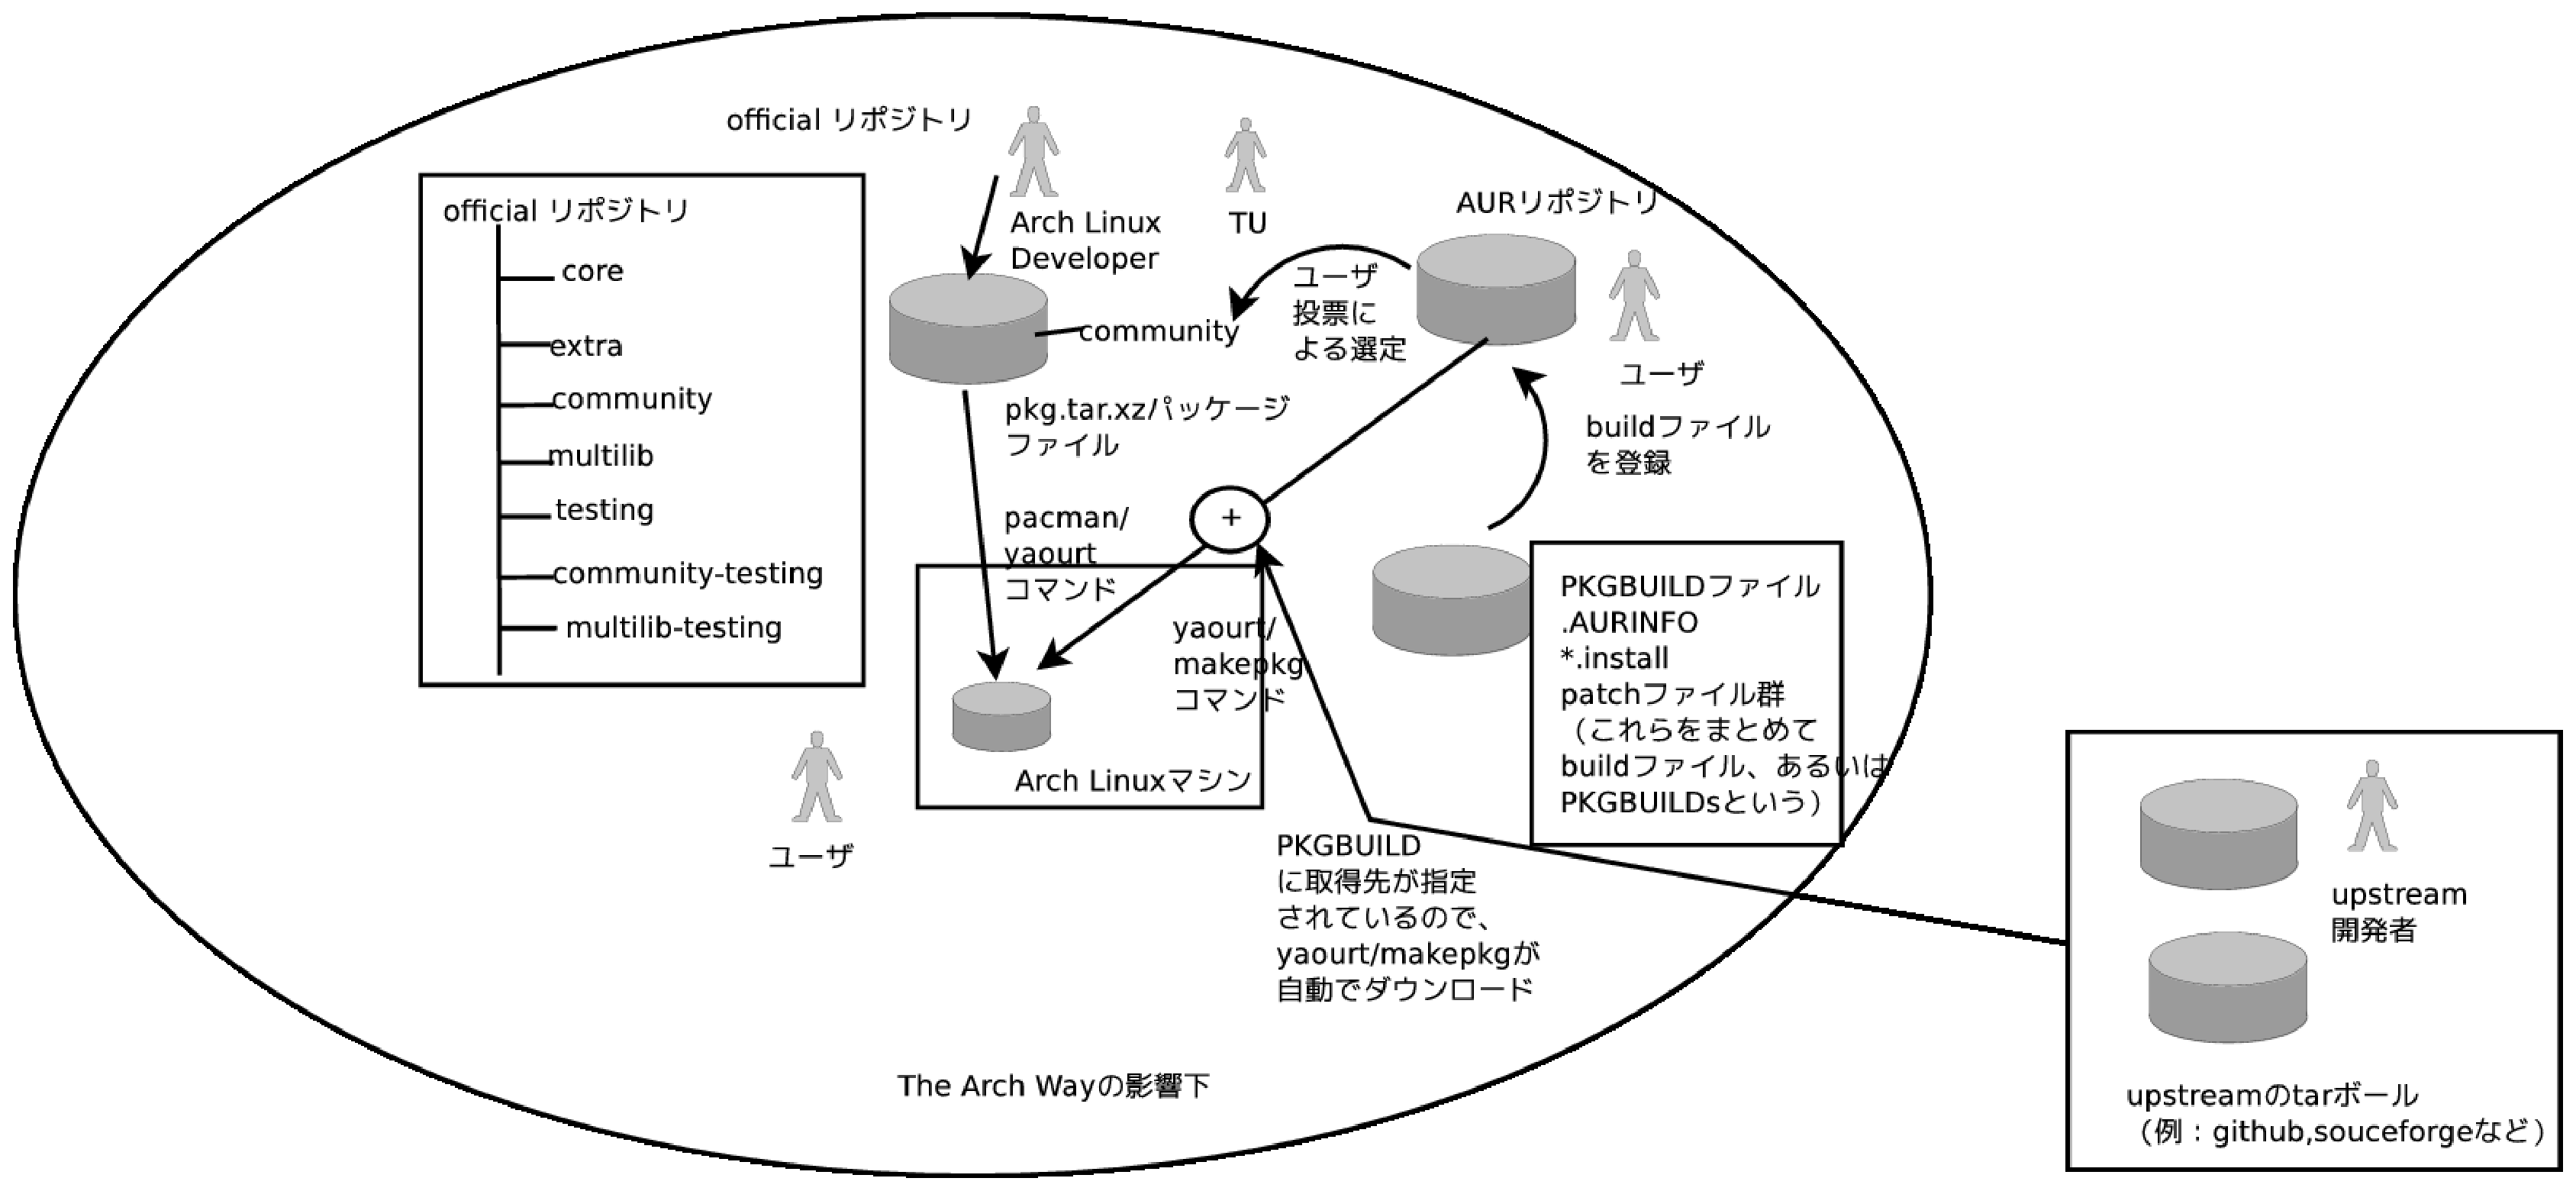
\includegraphics[width=0.8\hsize]{image201411/arch-schema_mono.eps}
 \caption{Arch Linux}\label{fig:arch-linux-schema}
\end{center}
\end{figure}

\subsection{AURとは}

 Arch Linuxには、officialリポジトリに含まれないソフトウェアについて、ユーザがPKGFILE等のbuildファイル一式をアップロードして他のユーザと共有して使うArch User Repository(AUR)というリポジトリが用意されています。AURから入手できるyaourt(ヨーグルトと読む)コマンドを使うと、AURをあたかもpacmanで扱ったかのように便利に使う事ができます。

 AURは、\url{https://aur.archlinux.org/}にて、アカウントを取得さえすれば、buildファイルを登録して公開できますので、非常に手軽に、新しいソフトウェア用のbuildファイルを他ユーザと共有して使うことができます。

 なお、AURはその使われ方から、登録されたbuildファイルは誰も精査していない場合があるため、基本的には自己責任(AT YOUR OWN RISK)での活用が求められます。

 AURに登録されたbuildファイルはユーザの投票により、一定量の支持が得られると、Trusted User(TU)らにより、officialリポジトリのcommunityリポジトリに取り込まれる仕組みのようです。

\subsection{Arch Linuxの良さ}

 使ってみてわかったArch Linuxの良さを列挙します。

\begin{itemize}
\item The Arch Wayに記載されているとおり、Arch Linuxを構成するあらゆるソフトウェアは最小限主義に貫かれています。従って、upstreamのソフトウェアとの変更点も最小としている為、設定ファイルの見通しが非常に良いです。
\item ユーザフレンドリということには重おきをおかず、ユーザの嗜好を極力邪魔しない(User Centerized)事をモットーとしているため、ユーザ自身が欲しいソフトウェアだけを導入という事がやりやすい作りになっています。
\item AURのように、利用者が自由にbuildファイルを登録できる仕組みがあるため、気軽にパッケージを公開することが出来ます。また、upstreamとの変更点を最小限に保つ方針のため、パッケージ化にかかる労力が少なくて済み、upstream側のリリースにあわせてスピーディーにパッケージ側のバージョンを追従させるが可能です。
\item 軽量です。パッケージを厳選して導入する事がしやすいため、マシンのスペックが低くても問題になりにくいです。
\end{itemize}

\subsection{終わりに}

 今回はArch LinuxとDebianを比較してみました。Arch Linuxはシンプルかつ最小限をモットーとしており、ソフトウェアの個別設定を自力で行う必要があります。そのため、Linuxシステムの勉強を熱心にしたい人、あるいは、導入するソフトウェアに強いこだわりがある人は、うってつけのシステムかと思います。

 その一方で、最初からある程度便利に使えるようにいろいろと自動で設定が行われ、マシン資源を消費するものの多くの便利なパッケージをある程度の量勝手に導入しておいてくれることを期待する人向けには、Debianの方がよくできています。

 Debianの良い所を正確に知る、あるいは目指すべき方向性の確認には、他のディストリビューションと比較することも重要かと思います。機会があれば、他のディストリビューションも使ってみて、Debianとの比較を行うのもよいのではないでしょうか。

\begin{thebibliography}{9}
\bibitem{ref:arch-linux-desc} Arch Linux (日本語), \url{https://wiki.archlinux.org/index.php/Arch_Linux_%28%E6%97%A5%E6%9C%AC%E8%AA%9E%29}
\bibitem{ref:arch-way} The Arch Way (日本語), \url{https://wiki.archlinux.org/index.php/The_Arch_Way_(%E6%97%A5%E6%9C%AC%E8%AA%9E)}
\bibitem{ref:history-arch-linux} History of Arch Linux (日本語), \url{https://wiki.archlinux.org/index.php/History_of_Arch_Linux_(%E6%97%A5%E6%9C%AC%E8%AA%9E)}
\bibitem{ref:arch-linux-install}Installation Guide (日本語), \url{https://wiki.archlinux.org/index.php/Installation_Guide_(%E6%97%A5%E6%9C%AC%E8%AA%9E)}
\bibitem{ref:debian-kvm} Debian wikiのKVMの章, \url{https://wiki.debian.org/KVM}
\bibitem{ref:arch-compare-other-dist} Arch Compared to Other Distributions (日本語), \url{https://wiki.archlinux.org/index.php/Arch_Compared_to_Other_Distributions_(%E6%97%A5%E6%9C%AC%E8%AA%9E)}
\end{thebibliography}

%201408 tokyo
%-------------------------------------------------------------------------------
\dancersection{Debianでタイルマップサービス作ってみた}{なかおけいすけ}
%-------------------------------------------------------------------------------
\index{debian-tilemap-service}

%NASA主催のInternational Space App Challengeという宇宙をネタにした
%アプリをつくるハッカソンで、地球観測衛星のデータを可視化してOpenStreetMapに
%オーバーレイできるタイルマップサービスを、Debianで開発しましたので紹介します。

\subsection{タイルマップサービスとは}
タイルマップサービス (TMS: Tile Map Service)は、OSGeo財団(Open Source Geospatial Foundation)が策定した、地図をタイルとして提供するプロトコルです。
タイルは、地図を領域とズームレベル毎に256px $\times$ 256pxの画像に分割した
もので、図\ref{fig:tile_pylamid}のようにピラミッド構造になっています。
大きな画像を小分割することで、必要な領域、ズームレベルだけを取得し、不要になった部分を
開放することで、メモリの消費量を削減し、効率良く通信を行うことができます。
タイルは、ズームレベルが一つ大きくなると、表示する範囲が$1/4$になります。
例えば、ズームレベル0では、地球全体を1枚のタイルで表し、ズームレベル1では4枚、
ズームレベル2では16枚....ズームレベルnでは$2^n \times 2^n$枚になります。
ズームレベル16になると、$2^{32} = 4,294,967,296 \simeq 4.3 \times 10^9$枚もの
タイルが必要になります。
%
\begin{figure}[hbp]
\centering

\includegraphics{image201408/Tiling.eps}
\caption{タイルのピラミッド構造\cite{ref:tile}}
\label{fig:tile_pylamid}
\end{figure}

タイルは、HTTPで、\texttt{http://BASEURL/VERSION/TILENAME/z/x/y.png} という形式のURIで取得できます。現在、VERSIONは1.0.0です。
ここでzはズームレベル、x、yは領域を表す整数です。x、yは、$lat$、$lon$を緯度、経度として
以下のように書けます\cite{ref:tilename}。
\begin{eqnarray*}
x &=& \frac{2^z(lon + 180)}{360}\\
y &=& 2^{z-1}(1-\frac{\ln(\tan(lat\frac{\pi}{180})) + \frac{1}{\cos(lat\frac{\pi}{180})}
}{\pi})
\end{eqnarray*}

\subsection{タイルの生成}
タイルを生成するためには、表示するデータが必要です。今回はJAXAの
水循環変動観測衛星「しずく」に搭載されているAMSR2というセンサーで観測された
海水表面温度データをタイルにしてみましょう。

「しずく」のデータは、登録が必要ですが一般公開されています\cite{ref:gcom_w1}。
登録をすると、sftpでデータをダウンロードできます。
%
\begin{commandline}
$ sftp -oPort=2051 username@gcom-w1.jaxa.jp
sftp> get AMSR2/YYYY/YYYY.MM/L3/SST_10/1/GW1AM2_YYYYMMDD_01D_EQOD_L3SGSSTHA1100100.h5.gz
\end{commandline}
%
ダウンロードしたファイルは、gzipで圧縮されたHDF5というファイルフォーマットの
数値データです。HDF5は科学技術用に開発された数値データを格納するためのバイナリーフォーマットで
多次元の数値データだけでなく、観測日時や観測者、スケーリングファクタ、解析アルゴリズムといった
情報を階層構造で格納することができるフォーマットです。もちろん仕様は公開されており
PythonやRubyのモジュールもあります。

この中に海水面温度の数値データが北緯0度、東経0度から0.1度刻みのメッシュで格納されています。
まずこのメッシュ1つを1pxとする画像を作ります。そうすると地球全体で3600px$\times$1800px
の画像ができます。

私はPythonを使って、メッシュのデータを取り出し、あらかじめ作っておいたカラーマップで
数値をRGBに変換し、ASCIIテキストでピクセルを表現できるPPMで出力しました。
欠損値は(R,G,B)=(0,0,0)としています。
\begin{figure}[hbp]
\centering

\includegraphics{image201408/map_mono.eps}
\caption{生成したマップ}
\label{fig:map}
\end{figure}

この画像をImageMagickのconvertコマンドでtiff画像にしつつ、欠損値を表す黒を
透明に変換します。
\begin{commandline}
$ convert -transparent black converted.ppm map.tiff
\end{commandline}

ここでできるTiff画像(図\ref{fig:map})は、地図ではありますが、ピクセルと緯度経度の対応関係の情報を持っていません。
そこでGDALを使って、このTiff画像を位置情報を持つGeoTiffというフォーマットに変換します。
GDALは、地理空間データのスイスアーミーナイフ的な存在で、
GeoTiffやJPG、PNGといったラスタデータフォーマットやHDF、NetCDF等のファイルを読んで
他のフォーマットに変換したり、測地系の変換等を行うことができるライブラリ、ユーティリティ群です。
(ここまででやってきた、HDF5ファイルから数値データを取り出してカラーマップにする
ことも、GDALだけでできる気がします。)
GDALは、gdal-binというパッケージになっています。TiffファイルをGeoTiffに変換するには、
gdal\_translate コマンドで、緯度経度が分かっているピクセルを教えてあげます。
そしてgdalwarpコマンドで、gdal\_translateで指定したピクセルと緯度経度を元に
幾何変換して測地系の情報を追加します。
%
\begin{commandline}
$ gdal_translate -q -gcp 0 0 0 90 \
                -gcp 3600 0 360 90 \
                -gcp 0 1800 0 -90 \
                -gcp 3600 1800 360 -90 map.tiff tmp.tiff

$ gdalwarp -q -s_srs EPSG:4326 -r cubic tmp.tiff map.tiff
\end{commandline}
%
各ピクセルが位置情報を持った画像ファイルが完成しました!
これでようやくタイルを生成する準備ができました。

タイルの生成には、python-gdalパッケージの gdal2tiles.py コマンドを使います。
ただこのコマンドは、指定したズームレベルのタイルをすべて生成してしまいます。
前述の通り、ズームレベルを増やすと指数関数的に生成する画像が増えていくので
タイルの生成に数時間かかってしまいます。
数時間かけて苦労してタイルを作っても、現実にはユーザーがすべてのタイルを
見てくれるわけではありません。だったら必要なタイルだけを、必要な時に生成すれば
良いのです。

\subsection{タイルマップサーバの実装}
では、リクエストがあったときに必要に応じてタイルを生成するサーバーを作りましょう。
今回はWebサーバはApacheで、mod\_pythonとmod\_rewriteを用います。
mod\_rewriteの説明は不要でしょう。正規表現にマッチしたリクエストのURLを
書き換えるモジュールです。

mod\_python は、ApacheのPython bindingで、CGIの置き換えを目的としたモジュールです。
インストールするには、以下のコマンドを実行します。
\begin{commandline}
# apt-get install libapache2-mod-python
# a2enmod python
# service apache2 restart
\end{commandline}
設定は、/etc/conf.d/ の中に適当なファイル名のファイルを作って
\begin{commandline}
<Directory /some/path>
  SetHandler mod_python
  PythonHandler mod_python.publisher
</Directory>
\end{commandline}
としすればよいでしょう。

mod\_pythonのmod\_python.publisherは、HTTPリクエストをPythonの
関数の呼び出しに変換します。
たとえば、www.example.org のDocumentRootに、hello.pyという
以下のPythonスクリプトがあったとしましょう。
\begin{commandline}
def sayHello(req, name):
  return ``Hello %s''%name
\end{commandline}
もしも、\url{http://www.example.org/hello.py/sayHello?name=Debian}にGET
リクエストがあると、Webサーバは、sayHello関数のname引数にDebianを代入して
sayHello関数を呼び出し、''Hello Debian''と表示されます。

タイルマップサービスにアクセスするクライアントは、
\url{http://BASEURL/VERSION/TILENAME/z/x/y.png}というURIでGETしようと
するので、mod\_rewriteでURIを書き換えましょう。たとえば、\url{www.example/org}の
/etc/apache/conf.dに以下のように設定すると、
%
\begin{commandline}
<Directory "/var/www/tile/1.0.0/sst">
    RewriteEngine   On
    RewriteBase     /tile/1.0.0/sst/
    RewriteRule     ^([0-9]+)/([0-9]+)/([0-9]+).png    gettile.py/get?z=$1&x=$2&y=$3

    AddHandler  mod_python    .py
    PythonHandler   mod_python.publisher
</Directory>
\end{commandline}
% $ <- for emacs font-lock
%
\url{http://www.example.org/tile/1.0.0/sst/4/12/34.png}が、
\url{http://www.example.org/tile/1.0.0/sst/gettile.py/get?z=4&x=12&y=34}
に変換されるので、gettile.pyの中の、req, x, z, yの引数をとる関数が呼び出されます。
ここに指定されたURIのタイルだけを生成処理を書けば、オンデマンドにタイルを生成する
タイルマップサービスができます。


単一タイルだけを生成するには、gdal2tiles.pyを少し修正します。
generate\_base\_tiles関数の中の
1180行目付近にすべてのタイルを作っているループが存在するので、

\begin{commandline}
     def generate_base_tiles(self):
         """Generation of the base tiles (the lowest in the pyramid) directl y from the input raster"""

                               (Snip...)

         for ty in range(tmaxy, tminy-1, -1): #range(tminy, tmaxy+1):
             for tx in range(tminx, tmaxx+1):

                 if self.stopped:
                     break
                 ti += 1
                 tilefilename = os.path.join(self.output, str(tz), str(tx), "%s.%s" % (ty, self.tileext))
                 if self.options.verbose:
                     print(ti,'/',tcount, tilefilename) #, "( TileMapService     : z / x / y )"
\end{commandline}

それをひも解いて指定されたタイルを生成している部分を、関数として抜き出します。
\begin{commandline}
     def generate_base_tiles(self):
         """Generation of the base tiles (the lowest in the pyramid) directl y from the input raster"""

                               (Snip...)

         for ty in range(tmaxy, tminy-1, -1): #range(tminy, tmaxy+1):
             for tx in range(tminx, tmaxx+1):
                 generate_tile(tx, ty, self.tmaxz)

     # -------------------------------------------------------------------------
     def generate_tile(self, ty, tx, tz):
         ds = self.out_ds
         tilebands = self.dataBandsCount + 1
         querysize = self.querysize
\end{commandline}

あとは、generate\_tile関数を、mod\_pythonが呼ぶスクリプトから呼べば
できあがりです。
\begin{commandline}
def get(req, z, tx, ty):
        req.content_type = 'image/png'
        #req.write('z: %s\ntx: %s\nty: %s'%(z,tx,ty))

        g = GDAL2Tiles(['/home/chome/public_html/tile/sst/map.tiff','/var/www/tile/1.0.0/sst'])
        g.open_input()
        g.generate_tile(int(ty),int(tx),int(z))

        with open('/var/www/tile/1.0.0/sst/%s/%s/%s.png'%(z,tx,ty), 'rb') as f:
                req.write(f.read())
\end{commandline}

\subsection{まとめ}
Debianでパッケージングされているオープンソースのプログラムやライブラリを組み合わせて
タイルマップサービスを作ってみました。
gdal2tiles.pyを少し修正しmod\_pythonから呼ぶことによって、オンデマンドで
必要なタイルだけを生成しています。

今回開発したサービスは\url{http://www.hi-rezclimate.org}で公開されています。
データの取得、GeoTiffにするところまでは自動化されているので、毎日最新のデータをダウンロードして自動で更新されています。「しずく」は海水面温度だけでなく、海上風速や水蒸気量、積雪深といった水に関する現象を観測しています。今後サポートするデータを増やしていく予定です。



\begin{thebibliography}{9}
\bibitem{ref:tile}``Tile Map Service in Geoide'', \url{http://geoikia.idgis.eu/wiki-english/index.php/Tile\_Map\_Services\_in\_Geoide}
\bibitem{ref:tilename} ``Slippy map tilenames'', \url{http://wiki.openstreetmap.org/wiki/Slippy\_map\_tilenames}
\bibitem{ref:gcom_w1} GCOM-W1 データ提供サービス \url{https://gcom-w1.jaxa.jp/auth.html}
\end{thebibliography}

%201406 kansai

\dancersection{Linuxのドライバメンテナになった体験記}{坂本貴史}

\subsection{今日の話題}

私は個人でサウンドデバイスドライバを書いています。そのコードが、サブシステム経由で、6月頭にLinux 3.16-rc1 にマージされました。サブシステムからLinuxにコードがpullされる流れを、実体験を基にして簡単にお話します。


\subsection{Linuxの開発サイクル}

「前の」、「今の」、「次の」バージョンと表現したとき、以下のようになります。

\begin{description}
\itemsep1pt\parskip0pt\parsep0pt
\item[0週]
前のバージョンをリリース。今のバージョンのマージウィンドウ開始。
\item[0〜2週]
この間、新機能がpullされる。
\item[2週]
マージウィンドウ閉鎖。今のバージョンのrc1をリリース。
\item[2週〜(N-1)週]
この間、バグ修正がpullされ、だいたい1週間おきにrcがリリースされる
\item[(N-1)週]
今のバージョンのrc(N-2)をリリース
\item[N週]
今のバージョンをリリース。次のバージョンのマージウィンドウ開始。
\end{description}

\subsection{Linuxのサブシステム}

機能別にサブシステムに分割されており、それぞれのサブシステムを開発するプロジェクトがあります。
\begin{multicols}{2}
\begin{itemize}
\item
  Scheduler
\item
  Memory management
\item
  Networking
\item
  Filesystems
\item
  Read-Copy update (RCU)
\item
  \ldots{}
\item
  IEEE1394 bus
\item
  Sound
\end{itemize}
\end{multicols}

\subsection{Linuxのサブシステムのメンテナ}

\begin{itemize}
\itemsep1pt\parskip0pt\parsep0pt
\item
  サブシステム内の開発をまとめる役割を果します
\item
  開発者から送られたパッチは、メンテナがマージするかどうかを決定します
\item
  マージウィンドウが開いたら、メンテナがLinusにpull requestを出します
\item
  Linusがrequestをackし、treeにマージします
\item
  メンテナはあらかじめ、Linusとの信頼関係を築いているため、拒否されることは珍しいようです
\end{itemize}

\subsection{Linuxの開発者の活動}

\begin{itemize}
\itemsep1pt\parskip0pt\parsep0pt
\item
  典型的には、サブシステム開発プロジェクトのメーリングリストで活動します
\item
  自分が書いたパッチのマージに向け、メンテナや他の開発者を説得します
\item
  RFC (Request for comment) を出し、他の開発者の反応を見ることが有効です
\item
  他の人が投げたパッチをレビューすると喜ばれます
\end{itemize}

\subsection{私がやったこと}
\begin{multicols}{2}
\begin{itemize}
\itemsep1pt\parskip0pt\parsep0pt
\item
  サウンドサブシステム
\item
  ALSA firewire stackの開発
\item
  firewireのプロトコルスタック
\item
  プロトコルスタックの実装
\item
  ドライバの実装
\end{itemize}
\end{multicols}

\subsection{開発の初期}

2013年1月〜2013年8月

目標は、デバイス仕様を把握することと、自分の活動をアピールすることです。

\begin{itemize}
\itemsep1pt\parskip0pt\parsep0pt
\item
  ライブラリモジュールの拡張
\item
  ドライバの作成
\item
  Linux firewire subsystemのバグ
\end{itemize}


\subsection{開発の中期}

2013年9月〜2014年1月

目標は、パッチセットの最終候補を作成し、テスターを募ることです。

\begin{itemize}
\itemsep1pt\parskip0pt\parsep0pt
\item
  別なデバイスチップの調査
\item
  ドライバのブラッシュアップ
\item
  既存実装のリグレッションテスト
\item
  最終RFCとCFT
\end{itemize}


\subsection{開発の後期}

2014年2月〜2014年6月

目標は、ALSAの上流にマージされるよう、コミュニケーションすることです。

\begin{itemize}
\itemsep1pt\parskip0pt\parsep0pt
\item
  影響のあるプロジェクトとの調整
\item
  3.14 のマージウィンドウの閉鎖
\item
  マージリクエスト 1 〜 3
\item
  3.15 のマージウィンドウの閉鎖
\item
  マージリクエスト 4
\item
  メンテナの緩い同意
\item
  topic/firewire ブランチ
\item
  0day kernel testing\footnote{0day kernel testing back-end (2012/05/17) https://lkml.org/lkml/2012/5/17/126} \footnote{KS2012: Kernel build/boot testing (2012/09/05) http://lwn.net/Articles/514278/}
\item
  testing backendのレポートへの対応
\item
  sound.gitのfor-nextへ
\end{itemize}


\subsection{マージ以降}

2014年6月

目標は、Linuxへのマージを見届けることです。

\begin{itemize}
\itemsep1pt\parskip0pt\parsep0pt
\item
  3.16 のマージウィンドウオープン
\item
  サブシステムメンテナからLinusへのプルリクエスト
\item
  コードの軽微な修正
\item
  サブシステムメンテナからLinusへのプルリクエスト
\item
  3.16 のマージウィンドウの閉鎖
\end{itemize}

\subsection{まとめ}

Linuxとそのサブシステムの間で、開発サイクルがどのように進められるかを、実体験を踏まえて説明しました。

\subsection{質問への回答}

\subsubsection{キャラクタデバイスとは何ですか?}

キャラクターデバイスとは、ユーザープロセスが、カーネルランドにあるコードを利用するためのエントリーポイントの一種です。ユーザープロセスがエントリーポイントに対して特定の操作を行なうと、カーネルランドにあるコードが実行され、ハードウェアとデータが交換されます。

一般的に、オペレーティングシステムは、ハードウェアの違いを吸収するレイヤを設け、同じプログラムルーチンで、同じ機能を持つ異なるハードウェアを扱えるようにしています。これにより、異なるハードウェアに対して異なるソフトウェアを書く必要がなくなるわけです。古い文献では、この機能を仮想マシン (virtual machine) と呼びます\footnote{「オペレーティング・システムの機能は、ユーザーに拡張マシン(extended machine)またはその下のハードウェアよりプログラムしやすい仮想マシン(virtual machine)を提供することであるといえる。」(ANDREW S. TANENBAUM (1989) 『MINIXオペレーティングシステム)』坂本文 監修、大西照代 翻訳、アスキー出版局)}。


この「仮想マシン」という文脈からキャラクタデバイスに言及すると、ハードウェアを抽象化してソフトウェアから利用できるようにしたもののひとつ、となります。

また一般的に、オペレーティングシステムは、複数のユーザープロセスが、擬似的に同時に走る機能を持ちます。これをTime Sharing Systemと呼びます。Time Sharing Systemは、ユーザープロセスがある条件を満たしたときあるいはシステムである事象が発生したとき、そのプロセスの実行を休止して状態を保存し、別なプロセスの状態を復元して実行を再開することで成立します。

Time Sharing Systemでは、様々なプロセスが、同時にシステム資源へアクセスすることがあります。そのためオペレーティングシステムは、システム資源に対するアクセスを管理する機能を持ちます。オペレーティングシステムは、ユーザープロセスに対し、ハードウェアへのアクセス方法をエントリーポイントに限定することで、システム資源を管理します。このシステム資源管理方法は、最近のメニーコア (CPUを複数持つ) マシンでも役に立ちます。

Linuxにおいて、大抵のエントリーポイントはファイルの形となっています。これはLinuxが、システムリソースをファイルで表現するというUNIXの設計思想に影響を受けているからです。キャラクタデバイスやブロックデバイスのエントリーポイントとなっているファイルを、特別に、「特殊ファイル ( special file)」と呼びます。ユーザープロセスは、基本的に、特殊ファイルに対してファイル操作を行い、ハードウェアとのデータ交換を行います。なお、このデータ交換を入出力 (input/output = I/O) と呼びます。

キャラクタデバイスは、バイト単位で入出力可能なハードウェアを表現します。身近なところでは、マウスやキーボードはキャラクタデバイスとなります(最も、これらはシステムへの入力限定、つまりキャラクタデバイスからの読み出し限定ですが)。Linuxにはこの他のエントリーポイントとして、ブロックデバイスがあります。固定サイズでデータを入出力可能なハードウェアを表現します。例えばハードディスクドライブが該当し、/dev/sda1となります。

さて、ユーザープロセスが特殊ファイルに対してファイル操作を行うと、システムコールが呼ばれてCPUの動作モードがユーザーモードからカーネルモードに変わり、ハードウェアにアクセスできるようになります。この時に実行されるコードのうち、カーネルランドにあるものをドライバと呼びます。キャラクタデバイスに対するドライバはキャラクタデバイスドライバ、ブロックデバイスに対するドライバはブロックデバイスドライバとなります。

Linuxのデバイスドライバにはこの他に、ネットワークデバイスドライバがあります。ネットワークデバイスドライバは他の2種類のドライバとは異なり、エントリーポイントがファイルではありません。ユーザープロセスは、専用の関数を実行し、ネットワークデバイスのエントリーポイントを取得します。このエントリーポイントに対する操作も、専用の関数となります。これら関数群をソケットインターフェイスと呼びます。

キャラクタデバイスおよびLinuxにおける他の2種類のデバイスに関して、オペレーティングシステムの基本機能やユーザープロセスからの利用方法も踏まえて説明しました。


\subsubsection{デバッグはどのように行いましたか?}

デバッグですが、printkなどのカーネルAPIでログを出力してカーネルスペースのデータ構造の状態を確認することと、簡単なプログラムを実行してデバイスの状態を確認することで行いました。便利なツールがたくさんありそうな気がしますが、私が気にしなければならないことに対して学習コストが高すぎると考えました。

私が書いたドライバの構造を簡単に述べると、下の方 (ボトムハーフ) はIEEE 1394バス上のユニット (デバイス) と入出力を行い、上の方 (トップハーフ) はALSA Coreを使ってユーザープロセスと入出力を行います。ドライバの仕事は、ALSA Coreがパターン化したユーザープロセスからの要求に合わせ、デバイスを操作し、特定の挙動をさせることです。ユニットに相当するスタブドライバを書くことも考えたのですが、Linux firewire subsystemが持つOHCI1394コントローラードライバをもうひとつ書くような大掛かりな仕事になるので、諦めました。

実はデバイスへの入出力は、ユーザースペースからも行うことができます。Linux firewire subsystemは、バス上にあるそれぞれのユニットに対してfwキャラクタデバイスを設け、libraw1394を通じてAPIを提供しています。デバイスの状態は、このAPIを利用する簡単なプログラムを実行して確認することができました。デバイスの挙動の調査は、だいたいこのユーザープログラムから行いました。

デバイスの挙動が明確になりさえすれば、あとはそれをC言語で書くだけです。gitでコードを管理し、コードの修正がある度にテストデバイスすべてを使って挙動を確認し、printkのログ出力で構造体の状態を確認するという作業がデバッグの中心でした。コードの分量が、個人がその実行パスを把握できる程度 (10,000行以下と言われています) だったのも幸いしました、

こうして振り返ってみると、kgdbを使ってカーネルスペースの構造体の確認をしたり、Linux firewire subsystemの学習のためにスタブドライバを書いたりするべきだったと思います。

%デバッグ方法について説明しました。

%201406 tokyo
%-------------------------------------------------------------------------------
\dancersection{GPG 秘密鍵取り扱い方法の提案}{吉田 晋}
%-------------------------------------------------------------------------------
\index{gpg-private-keys-store-and-maniplate}

\subsection{はじめに}

皆さん、GPG のキーサインパーティーに参加した事ありますか?
私は、昨年の大統一 Debian 勉強会 2013 で初めて参加し、GPG の秘密鍵も、その時初めて作りました。
ところで、この秘密鍵はどのように保管すれば良いのでしょうか?

鍵はいつでも再発行出来るとはいえ色々と手間がかかりますし、古い鍵で暗号化したファイルを複合化出来なくなると困ります。
記録メディアの破損による鍵のロストには要注意です。
一般的に、記録メディアの破損に備えるには複数のメディアを複数の場所で保存する事は良い方法です。

一方、最低限のマナーとして盗難にも気をつける必要が有るでしょう。
厳重に管理するには、バックアップの数は少ないほど有利です。

さて、メディア破損に備えて冗長性を持たせる方法と盗難に備えて厳重に管理する方法は真っ向から矛盾してしまいました。
結局、どうすれば良いのでしょう?

\subsection{アイディアのベースは RAID}

例えば 3 本のディスクを用いた RAID5 のディスクアレイでは、2 個のディスクにデータを分散して記録しながら残りの 1 個のディスクにパリティデータを保存します。
同じ要領で秘密鍵を 2 個のファイル + 1 個のパリティファイル = 計 3 個のファイルを PC、USB メモリ(肌身離さず)、DVD(金庫)の 3 カ所で保存すれば、
\begin{itemize}
\item 普段は、USB メモリと PC を使って、都度鍵ファイルを復元して使用

  (使用後は鍵ファイル削除。削除忘れ防止のため、tmpfs 上で作ると良いかも。)
\item PC や USB メモリが盗まれても、しばらくは安全
\item ディスクのクラッシュや USB メモリの破損時には金庫の DVD を使って復元
\end{itemize}
という冗長性と秘匿性を兼ね備えた状態に成ります。
完全な鍵を世界中のどこにも保存する必要が無いところがポイント高!

\begin{figure}[H]
\begin{center}
  \begin{tikzpicture} [x=1em, y=1ex]
    \draw (-7, 0) rectangle (7, -24.5);
    \draw (0, -3) node {秘密鍵};
    \draw [red] (-3.8, -7.5) rectangle (3.8, -13.5);
    \draw (0, -9) node {1 0 0 0 1 1 ...};
    \draw (0, -12) node {......};
    \draw [blue] (-3.8, -17) rectangle (3.8, -23);
    \draw (0, -18.5) node {0 0 1 1 1 0 ...};
    \draw (0, -21.5) node {......};

    \draw [red] (-23, -30.5) rectangle (-9, -42.5);
    \draw (-16, -33) node {PC のディスクで保持)};
    \draw (-16, -36) node {1 0 0 0 1 1 ...};
    \draw (-16, -39) node {......};

    \draw [blue] (-7, -30.5) rectangle (7, -42.5);
    \draw (0, -33) node {USB メモリで肌身話さず};
    \draw (0, -36) node {0 0 1 1 1 0 ...};
    \draw (0, -39) node {......};

    \draw [green] (9, -30.5) rectangle (23, -42.5);
    \draw (16, -33) node {金庫で保管(parity)};
    \draw (16, -36) node {1 0 1 1 0 1 ...};
    \draw (16, -39) node {......};
  \end{tikzpicture}
\caption{分散管理イメージ図}
\end{center}
\end{figure}

ちなみに、分散するファイルの数を 2 倍にしたらどうなるでしょう?
秘密鍵を 4 個のファイル + 2 個 = 計 6 個のパリティファイルに分散すれば、パリティ増による冗長性の向上と、ファイル 1 個あたりの情報量減による秘匿性の向上を両立可能です。

\subsection{プロトタイプ作ってみた}

プロトタイプは Python 2.7 で作成し、 Debian Sid で動作確認を行いました。

dVault (distribute vault) と命名
\vspace{1cm}

\url{https://github.com/wbcchsyn/dVault_prototype}

(src/dvault が本体)
\vspace{1cm}

\subsubsection{注意}

あくまでプロトタイプなので、絶対に自分の秘密鍵に対して使わないで下さい。

例えば、
\begin{itemize}
\item 作成したファイルのパーミッションとか、全然気にしてません。
\item 問答無用でファイルの上書きをします。

  秘密鍵を上書きしながら途中で失敗すると、秘密鍵が失われます。
\end{itemize}
\vspace{1cm}

\subsubsection{使用方法}

origin というファイルを split0, split1, parity の 3 個のファイルに分割する場合

\begin{commandline}
$ dvault split -u origin -s split0 -s split1 -s parity
\end{commandline}

split0, parity の 2 個のファイルから origin を復活させる場合

\begin{commandline}
$ dvault unite -u origin -s split0 -s split1 -s parity
\end{commandline}
\vspace{1cm}

\subsubsection{仕様}
\begin{itemize}
\item パリティは 1 個で固定
\item 分散した各ファイルの最初にはメタ情報を json で保存。

  その後に 1 行空行を入れて、実際のデータを記入

  とりあえず、メタ情報は以下の 3 個 \begin{itemize}
  \item united\_length 元ファイルの長さ
  \item split\_count 何個に分割したか。(最低 2。)

    この数とパリティファイル 1 個、最低 3 個のファイルが出来る
  \item index 何番目のファイルか。(0 始まり。)

    index = split\_count の時は、パリティファイル
  \end{itemize}
\item 元ファイルを 1 byte ずつ分割。

  united\_length が split\_count で割り切れない場合は 0 でフィリング
\item 最後のファイル書き出し時以外は全てオンメモリで処理。

  一時ファイルは作りません
\end{itemize}
split\_count = 2 の場合、奇数目 byte を index = 0 のファイルに、偶数目 byte を index = 1 のファイルに、パリティ情報を index = 2 のファイルに保存

\subsection{実演}
\subsubsection{分割}

中身が \verb|abcedf\n| の 7 byte のファイルを 2 個 + parity の計 3 個に分割してみる
\vspace{1cm}

\begin{commandline}
$ hexdump -C origin

00000000  61 62 63 64 65 66 0a                              |abcdef.|
00000007

$ dvault split -u origin -s split0 -s split1 -s parity

$ hexdump -C split0

00000000  7b 22 69 6e 64 65 78 22  3a 20 30 2c 20 22 75 6e  |{"index": 0, "un|
00000010  69 74 65 64 5f 6c 65 6e  67 74 68 22 3a 20 37 2c  |ited_length": 7,|
00000020  20 22 73 70 6c 69 74 5f  63 6f 75 6e 74 22 3a 20  | "split_count": |
00000030  32 7d 0a 0a 61 63 65 0a                           |2}..ace.|
00000038

$ hexdump -C split1

00000000  7b 22 69 6e 64 65 78 22  3a 20 31 2c 20 22 75 6e  |{"index": 1, "un|
00000010  69 74 65 64 5f 6c 65 6e  67 74 68 22 3a 20 37 2c  |ited_length": 7,|
00000020  20 22 73 70 6c 69 74 5f  63 6f 75 6e 74 22 3a 20  | "split_count": |
00000030  32 7d 0a 0a 62 64 66 00                           |2}..bdf.|
00000038

$ hexdump -C parity

00000000  7b 22 69 6e 64 65 78 22  3a 20 32 2c 20 22 75 6e  |{"index": 2, "un|
00000010  69 74 65 64 5f 6c 65 6e  67 74 68 22 3a 20 37 2c  |ited_length": 7,|
00000020  20 22 73 70 6c 69 74 5f  63 6f 75 6e 74 22 3a 20  | "split_count": |
00000030  32 7d 0a 0a 03 07 03 0a                           |2}......|
00000038
\end{commandline}

\subsubsection{リストア}

フィアル split1、origin を無くしたとして、split0、parity から origin を復活させる
\vspace{1cm}

\begin{commandline}
$ rm origin split1

$ dvault unite -u origin -s split0 -s parity

$ hexdump -C origin

00000000  61 62 63 64 65 66 0a                              |abcdef.|
00000007
\end{commandline}

\subsection{悩み}
\begin{itemize}
\item Python で実装したが、果たして良かったのか?

  Debian の最小構成で Python が入っていない

  パッケージ化を目指すなら、C で再実装した方が良いかも
\item メタ情報を json で保存して良かったのだろうか?

  今後メタ情報が増えた場合に、文字列と数字の区別が出来たら便利だと思って json にした。

  しかし、C で実装する場合は json のパースは面倒。

  何より、現状では json の中で改行 x 2 が入ったらバグるので何とかする必要あり。
\item オンメモりの処理にどこまでこだわるか?

  OS 上のファイルとしては存在しなくとも、ディスクに少しでもデータが残ると盗難時に解析される恐れがあるのでオンメモリの処理にこだわった。

  でも、よく考えると SWAP したら意味が無いし、最初に秘密鍵を生成する際にディスク上に一時保存したら終わり。

  大容量のファイルを分割する事に備えて、名無しの一時ファイル(開いた直後に OS で削除)くらいは使っても良いかも。
\item 複数パリティに対応した方が良いか?
\end{itemize}

\subsection{今後の予定}

自分以外の人が使ってくれるなら、メンテナンスを行うつもりです。

(ドキュメントも作成する必要あり)

「使ってみたい」という人がいらしたら、教えて下さい。

%201407 tokyo
%-------------------------------------------------------------------------------
\dancersection{JenkinsでのDebianパッケージ自動化}{前田耕平}
%-------------------------------------------------------------------------------
\index{building-packages-automatically-on-jenkins}

昨年の大統一Debian勉強会2013で、「とある企業でのDebianシステムの使い方。」というセッション\footnote{\url{http://gum.debian.or.jp/2013/session/437.html}}の中で、社内向けのDebianパッケージの作成と、repreproを使ったパッケージの配布方法についての話をしました。今回はその続編です。

\subsection{背景}

管理するパッケージが少ない場合は、手作業でのビルドでも間に合っていましたが、管理するパッケージ数が増え、対象ディストリビューションが増え(Precise, Wheezy, Trusty)、一方メンテナンスする人を増やすのは時間が掛かる、という状況でした。

そこで、別件\footnote{JavaやPythonのプロジェクトのビルドやテストの実行目的。}でJenkinsを用意したこともあったので、ソースパッケージを作成するプロセス以外は、全てJenkinsで実行して自動化することにしました。

\subsection{自動化するプロセス}

パッケージのビルドからローカルアーカイブへの登録までに行うプロセスは図1のようになります。
1aは公式パッケージのソースパッケージをdgetなどで取得する場合、1bは独自にソースパッケージを作成する場合です。ビルドする対象のソースパッケージによって実際の手段自体は異なってきますが、実行するプロセス自体は図の通り変わりません。

\begin{figure}[H]
\begin{center}
\begin{tikzpicture} [x=1em, y=1ex]
  \draw (-33, -1) rectangle (-17, -5);
  \draw (-25, -3) node {1a. ソースパッケージ取得};
  \draw[->] (-25, -5) -- (-17, -8);

  \draw (-5, -1) rectangle (11, -5);
  \draw (3, -3) node {1b. ソースパッケージ作成};
  \draw[->] (3, -5) -- (-5, -8);

  \draw (-23, -8) rectangle (1, -12);
  \draw (-11, -10) node {2. パッケージビルド};
  \draw[->] (-11, -12) -- (-11, -15);

  \draw (-23, -15) rectangle (1, -19);
  \draw (-11, -17) node {3. パッケージチェック};
  \draw[->] (-11, -19) -- (-11, -22);

  \draw (-23, -22) rectangle (1, -26);
  \draw (-11, -24) node {4. インストールテスト};
  \draw[->] (-11, -26) -- (-11, -29);

  \draw (-23, -29) rectangle (1, -33);
  \draw (-11, -31) node {5. ソースパッケージへの署名};
  \draw[->] (-11, -33) -- (-11, -36);

  \draw (-23, -36) rectangle (1, -40);
  \draw (-11, -38) node {6. ローカルアーカイブへの登録};
\end{tikzpicture}
\caption{パッケージビルド〜ローカルアーカイブへの登録までのプロセス}
\end{center}
\end{figure}

各プロセスの実行内容は下記のようになります。

\begin{figure}[H]
\begin{center}
\begin{tikzpicture} [x=1em, y=1ex]
  \draw (-33, -1) rectangle (-17, -5);
  \draw (-25, -3) node {1a. dgetで公式アーカイブから取得};
  \draw[->] (-25, -5) -- (-25, -8);

  \draw (-5, -1) rectangle (11, -5);
  \draw (3, -3) node {1b. git-buildpackageでGitで管理};
  \draw[->] (3, -5) -- (3, -8);

  \draw (-33, -8) rectangle (-17, -12);
  \draw (-25, -10) node {2a. cowbuilder/pbuilderでビルド};
  \draw[->] (-25, -12) -- (-17, -15);

  \draw (-5, -8) rectangle (11, -12);
  \draw (3, -10) node {2b. git buildpackageでビルド};
  \draw[->] (3, -12) -- (-5, -15);

  \draw (-23, -15) rectangle (1, -19);
  \draw (-11, -17) node {3. ビルド時のhook scriptとしてlintianでチェック};
  \draw[->] (-11, -19) -- (-11, -22);

  \draw (-23, -22) rectangle (1, -26);
  \draw (-11, -24) node {4. piupartsでインストール&アンインストールテスト};
  \draw[->] (-11, -26) -- (-11, -29);

  \draw (-23, -29) rectangle (1, -33);
  \draw (-11, -31) node {5. debsignで署名};
  \draw[->] (-11, -33) -- (-11, -36);

  \draw (-29, -36) rectangle (7, -43);
  \draw (-11, -38) node {6-1. dputでincomingディレクトリにpush};
  \draw (-11, -41) node {6-2. dputのpost\_upload\_commandとしてreprepro processincommingを実行};
\end{tikzpicture}
\caption{各プロセスの実行内容}
\end{center}
\end{figure}

これらをJenkinsでジョブとして実行するためには、
対話形式の処理をなくし、リモートホスト上の処理も実行可能な状態で、
一連の処理をJenkinsのジョブスクリプトを作成する必要があります。

\subsubsection{Jenkinsで実行する上での課題}

Jenkinsで実行する上で問題となるのは、GPGとSSH公開鍵のパスフレーズの入力と、
repreproでのアーカイブの登録です。

repreproでのアーカイブ登録は\texttt{reprepro processincoming}コマンドで行います。Jenkinsと別ホストでrepreproを実行する場合、dput.cfの\texttt{post\_upload\_command}を使えば解決できます。
例えば、Ubuntu Trusty用のローカルアーカイブにdputする場合は、下記のような設定をdput.cfにしておきます。

\begin{commandline}
[trusty]
fqdn                    = repo.example.org
method                  = scp
incoming                = /var/lib/debpkg-custom/ubuntu/incoming/
login                   = repoadm
post_upload_command     = ssh repoadm@repo.example.org /usr/bin/reprepro -b /var/lib/debpkg-custom/ubuntu \
--keepunreferencedfiles processincoming trusty #実際は一行
\end{commandline}

公開鍵の入力は、次の3箇所で必要になります。\footnote{Jenkinsとrepreproを同じホストで実行する場合(つまり一台で完結させる場合)にはSSH公開鍵のパスフレーズ入力は特に考慮することはありません。}

\begin{itemize}
  \item GPG
    \begin{itemize}
    \item[5.] debsignでの署名
    \item[6-2.] dputのpost\_upload\_commandとしてreprepro processincommingを実行
    \end{itemize}
  \item SSH
    \begin{itemize}
    \item[6-1.] dputでincomingディレクトリにpush
    \end{itemize}
\end{itemize}

一方、GPGについては既存環境で使っている鍵をそのまま利用する関係上、避けて通れません。
Jenkinsのジョブスクリプトで

\begin{commandline}
$ echo -e 'passphrase\npassphrase\n' | debsign some.changes
$ echo -e 'passphrase\npassphrase\n' | dput some.changes
\end{commandline}

と実行しても標準入力からはパスフレーズは渡せません。しかし、gpgコマンド自体には\texttt{--no-tty --batch}オプションを使って、対話形式でなくてもパスフレーズを入力することができます。そのため、方法としては、
\begin{itemize}
  \item debsign, reprepro processincommingをTTYなしで対話形式でなくてもGPGパスフレーズを入力できるようにする
  \item expectを使ってプロンプトで判断してパスフレーズを入力させる
\end{itemize}

の2つの方法が考えられます。
で、先に着手したdebsignについては、expectで処理するのは負けだと思ったので、別途pydebsignというPythonライブラリを実装しました\footnote{Git: \url{https://github.com/mkouhei/pydebsign}, PyPI: \url{https://pypi.python.org/pypi/pydebsign}}。しかし、repreproについては時間の都合上、結局Python版のexpectのpexpectを使いました。下記のようになります。\footnote{debsignのこれで良かったですね。。。}

\begin{commandline}
def upload_files(codename, changes_path, reprepro_passphrase):
    """ uploading to local archive incoming directory of reprepro """
    os.environ['LANG'] = 'C'
    command = "dput %s %s" % (codename, changes_path)
    exp = pexpect.spawn(command, maxread=4000)
    exp.logfile_read = sys.stdout
    exp.expect('Please enter passphrase:')
    exp.sendline(reprepro_passphrase)
    exp.expect('Please enter passphrase:')
    exp.sendline(reprepro_passphrase)
    exp.expect(pexpect.EOF)
    exp.close()
    return exp.status
\end{commandline}

\subsubsection{Jenkinsで必要なプラグイン}

パスフレーズは渡せるようになりましたが、Jenkinsのジョブを実行するとパスフレーズが丸見えです。そのため、"Mask Passwords Plugin"\footnote{\url{https://wiki.jenkins-ci.org/display/JENKINS/Mask+Passwords+Plugin}}というプラグインを使います。
他に必要なプラグインは下記の通りです。また、Jenkinsのジョブスクリプト管理用と、git-buildpackage用と複数のGitリポジトリを扱えるようにするため、"Git Plugin"\footnote{\url{https://wiki.jenkins-ci.org/display/JENKINS/Git+Plugin}}と"Multiple SCMs Plugin"\footnote{\url{https://wiki.jenkins-ci.org/display/JENKINS/Multiple+SCMs+Plugin}}も必要です。これらのプラグインは後述のJenkins環境構築後に、Jenkinsの管理画面からインストールします。

\subsubsection{その他の考慮点}
\begin{itemize}
\item Jenkinsで自動ビルド&ローカルアーカイブへ登録したパッケージに依存するパッケージを作成することもあります。そのため、後述のpbuilderとcowbuilderのイメージのAPT lineには、ローカルアーカイブのURLを登録し、ローカルアーカイブの公開鍵をapt-keyで登録しておく必要があります。
\item バックポートする場合、orig.tar.{gz,xz}が.changesファイルのリストにはデフォルトでは登録されず、repreproで登録する際にエラーになります。そのため、debbuildopts='-sa'を指定する必要もあります。
\item pbuilderやcowbuilderでパッケージをビルドすると、デフォルトでは/var/cache/pbuilder/resultsディレクトリ以下に作成されます。このままでは、Jenkinsのジョブごとに処理するには不都合です。pbuilderrcでBUILDRESULTに、Jenkinsのworkspace以下のパスを指定するようにします。
\end{itemize}

以上の点を考慮し、PythonでJenkinsジョブ用のスクリプトを作成しました。\footnote{デモのみ。}
都合により、Golang版も作成しました。\footnote{\url{https://github.com/mkouhei/godebbuild}}
これらは、前述のhook scriptで行うlintianでのテストを、dputの\texttt{-l}オプションで実行できるようにしています。\footnote{backportなどの場合、lintianのWarning, Errorを修正するためのパッケージの変更せず、許容してしまいたいこともあるため。}

\subsection{Jenkins及びreprepro環境の構築}

Jenkinsで自動実行するための環境として、下記の準備が必要になります。

\begin{itemize}
  \item Jenkinsのインストール&設定
  \item Jenkins用ユーザへのsudo設定
    \begin{itemize}
      \item /usr/sbin/pbuilder
      \item /usr/sbin/cowbuilder
      \item /usr/bin/git-buildpackage
      \item /usr/bin/piuparts
      \item /bin/chown
    \end{itemize}
  \item pbuilder and cowbuilderイメージの作成
    \begin{itemize}
      \item ビルド対象のディストリビューションの数分だけ作成
    \end{itemize}
  \item debsignおよびreprepro用のGPG鍵の作成
  \item repreproへのupload用のSSH公開鍵の作成\footnote{Jenkinsとrepreproが別ホストの場合}
  \item dput.cfの設定
  \item rererproのインストール&設定
  \item reprepro管理poolの公開設定
  \item ローカルアーカイブ用のGPG公開鍵のexport
\end{itemize}

このうち、pbuilderとcowbuilderイメージの作成の一部と、GPG鍵の作成、SSH公開鍵の作成については、手動で行う必要がありますが、他はAnsibleで自動化しました。\footnote{デモ参照。Playbookは、\url{https://github.com/mkouhei/playbook-tokyodebian115}に用意してあります。}

\subsection{まとめ}

ソースパッケージの作成とJenkinsのジョブの作成以外は自動化できました。
これにより、Debianパッケージの作成をやったことが無い人でもバックポートなどはできるようになりました。
しかし、実際にはジョブを実行するとパッケージの依存関係や、lintian、piupartsなどのエラーが発生します。そのため、Debianパッケージ作成について知らなければ、それらのエラーに対応できないことが予想されます。

また、ソースパッケージの作成は相変わらず、属人化しています。\footnote{つまり、職場では自分しか作成できない。}
なので、今回のDebianパッケージング道場でパッケージ作成ができる人が増えるとイイですね。\footnote{原稿作成時点では職場の同僚の参加者は未定。}

%201409 tokyo
%-------------------------------------------------------------------------------
\dancersection{DebConf14のビデオ紹介}{野島 貴英}
%-------------------------------------------------------------------------------
\index{debconf14-video-intro}

\subsection{DebConf14}

 DebConfとは毎年1回Debian Project主催で開かれる大きなカンファレンスのことです。

 そこでは、世界中からDebian Projectの活動に興味を持つ方々が集まり、Debianの開発や貢献についての
発表や活発な議論が行われています。

 今年は第15回目のカンファレンスとなり\footnote{DebConf0が存在するので、全部で15回目です。}、8/23〜8/31の間、米国オレゴン州ポートランドにて、DebConf14と
して開かれました。

 ここでは、DebConf videoチームにより公開されているDebConf14のカンファレンスの各セッションのビデオ
を視聴し語ってみます。

\subsection{DebConf14のビデオに関する情報}

 DebConf14のスケジュールと、開かれたセミナの概要などの情報は、DebConf14の公式ホームページの\url{http://debconf14.debconf.org/}を見て下さい。

 セミナとBOFの動画ファイルは、\url{http://meetings-archive.debian.net/pub/debian-meetings/2014/debconf14/webm/}にwebmフォーマットでおいてあります。video codecはvp8、audio codecはvorbisという、Debianらしくオープンな技術に拘ったデータ形式となっているのが特徴です。

\subsection{視聴するにあたって補足}

 大量のビデオが公開されており、また時間も1時間弱程度はあるので、きっと本勉強会にいらっしゃるような熱心なDebian関係者の方は、
そのままのスピードで視聴するのではなく、早回しで視聴したいという要望を持たれる方がいらっしゃると思います。そんな時には、
mplayer2をお勧めしておきます。

\begin{commandline}
$ apt-get install mplayer2
$ mplayer2 <動画ファイル名>
\end{commandline}

 また、起動するとわかるのですが、あまり親切なメニューは出てきません。代わりにman mplayerするとわかるのですが、
豊富なショートカットキーがあり、こちらを使う事により再生を制御できます。(表\ref{tab:mplayer-key}参照)


\begin{table}[htbp!]
\centering
\begin{tabular}{|l|p{7cm}|l|p{7cm}|}
\hline
キー&操作 &キー & 操作\\ \hline \hline
[ & 10\%スロー & ] & 10\%スピードアップ \\ \hline
$\leftarrow$ & 1分戻し & $\rightarrow$ & 1分スキップ \\ \hline
$\uparrow$ & 10分戻し & $\downarrow$ & 10分スキップ \\ \hline
o & 残り時間/再生時間表示(複数回押す) & q & mplayerを終了\\ \hline
\end{tabular}
\caption{mplayerのショートカットキー}
\label{tab:mplayer-key}
\end{table}

 また、英語の聞き取りが苦手な方には、DebConf subtitle projectらによる、英語による書き起こしのテキストデータが入手できます。
gitからの入手の仕方は以下のとおりです。

\begin{commandline}
apt-get install git
git clone http://anonscm.debian.org/git/debconfsubs/debconfsubs.git
cd debconfsubs/2014/debconf14/english/wip/
\end{commandline}

 2014/9/25現在のところ、未完成のものも含めて9つのセッションに関する書き起こしデータが手に入るようです。
なお、.srtの拡張子を持つデータは字幕データであり、字幕ファイルを扱える動画プレイヤーで字幕を表示しながら
セッションの動画を視聴することが出来ます。こちらについての操作方法の例は、第105回東京エリアDebian勉強会のセミナ
資料\cite{ref:osc-tokyo-2013-fall}に具体的に記載していますので、こちらを参考にしてください。

 さらに、gitに格納されるよりも早く字幕の英文を見たい、あるいは、そもそも自分で英文字幕を起こす手伝いをしたい人は、
\url{https://wiki.debconf.org/wiki/Videoteam/Subtitles}で紹介されている\url{http://www.amara.org/}
の字幕書き起こし用のWEBサービスにアクセスしてください。こちらのページから起こし途中の字幕を閲覧したり、
字幕付きのDebConf14のセッションの動画を実際に見ることが出来ます。

\subsection{DebConf14大物ゲスト}

 今回は、Debianに直接の関係はあまりないのですが、大物ゲストが呼ばれており、専門のセッションが開かれています。

 \subsubsection{Q\&A with Linus Torvalds}

\begin{wrapfigure}{r}{5cm}
  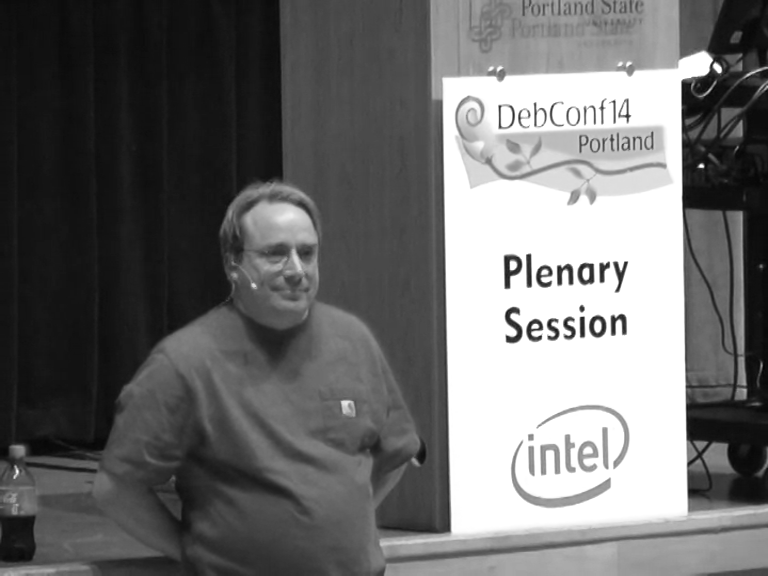
\includegraphics[width=5cm]{image201409/qa_linus_mono.png}
\end{wrapfigure}

  Linuxカーネルの最初の作者であるLinus Toravalds本人を呼んで、セミナ参加者から一人づつ質問を受け続けるというセッションです。

 \begin{itemize}
  \item Linusさんの関心のほとんどはLinuxカーネルそのものに費やされており、ディストリビューションの動向についてはあまり気にしてないようです。
Debianも1度試したきりで結局Macに入れようとして失敗しただけのようで(Ubuntuも同様)。
  \item gccの件や、systemdの件など、次々と一見答えにくい(?)質問が次から次へとLinusさんにぶつけられていました。特にsystemdの件ではLinusさんもコミュニティでの扱いについて熱い答弁をされていました。
  \item GPUとkernelの関係などについて昨今の事情についての質問もありました。
  \end{itemize}

 最初の質疑でLinusさんも非常に気楽に答えていたためうっかり、品位に欠ける表現がところどころ飛び出してしまい、女性のDebConfスタッフ(Debian Womenの方)に表現の注意を受ける一幕もありました。

 \subsubsection{Weapons of the Geek}

\begin{wrapfigure}{r}{5cm}
  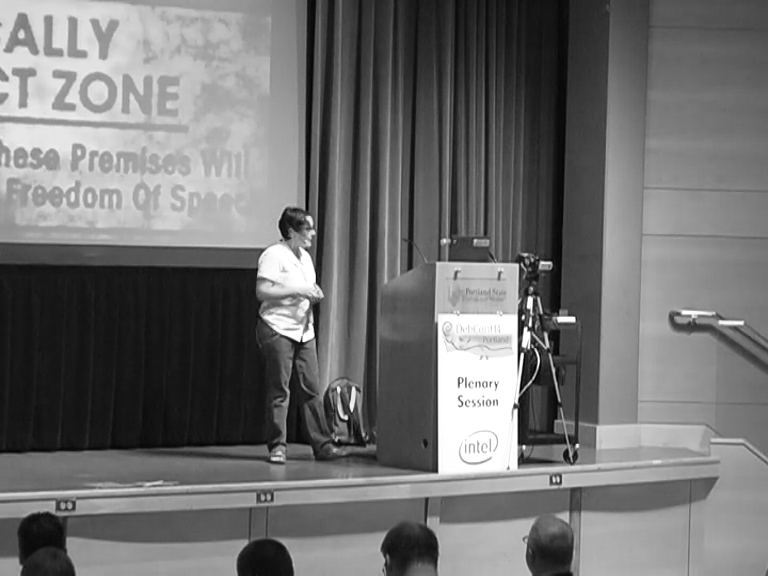
\includegraphics[width=5cm]{image201409/weapon_geek_mono.png}
\end{wrapfigure}

 クラッカー集団であるAnonymousについての社会面、文化面の研究で有名な、Gabriella Colemanさんのセッション。AnonymousとAnonymousを取り巻く独特のハッカー文化の解説と考察を行うというセッション。日本にはほとんど馴染のないサブカルチャー(例:XENU,Chanology,Scientologyなど)の紹介と、これらに対するAnonymousの考え方への影響などの紹介があって面白いです。

\subsection{Debianの主なトピック}

\subsubsection{Bit From the DPL}

\begin{wrapfigure}{r}{5cm}
  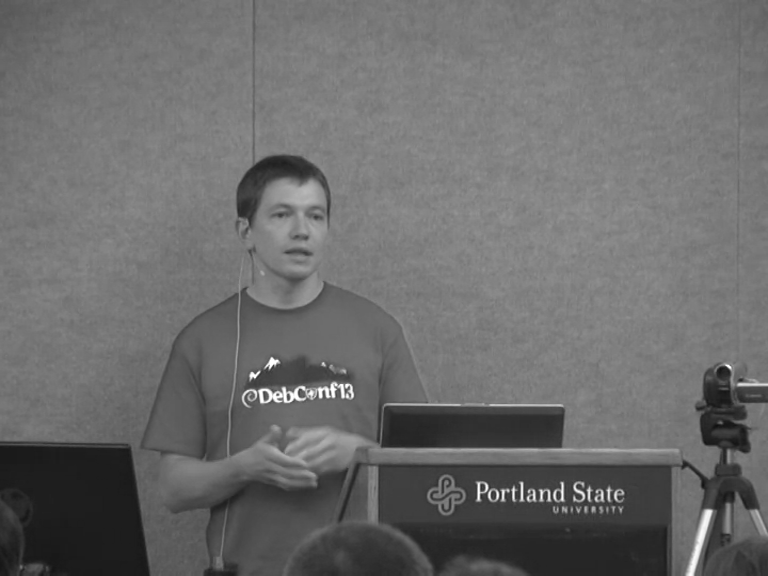
\includegraphics[width=5cm]{image201409/bit_dpl_mono.png}
\end{wrapfigure}

 2014年もDPL続投のLucas Nussbaumさんのプレゼン。

 プレゼン資料は、\url{http://blop.info/p/201408-dc14-dpl.pdf}で公開中。

 \begin{itemize}
 \item Debian Projectの収支の件の話が出ました。Debian Projectは資産をTrusted Organizationとして認めた機関にあずけているのですが、全部あわせると、日本円で約2,800万円ぐらいある模様です。保有割合としては、SPI(米国/US\$預かり)が最も多い状況です。さらに、DebConfの度にスポンサーからの寄付を使い切れず資産が増えてしまう模様で、ここ2年がその傾向が顕著とのことです。
 \item さらなる予算の活用についてのディスカッションが行われました。予算利用の候補としての案は以下の4つ。
   \begin{enumerate}
      \item Debianの普及に使う(例:mini-DebConfをもっと開く。景品(Tシャツなど)を新しい貢献者へ配る、Debianのブースの何かに使う)
      \item セキュリティに関して強化。Debian公式開発者へ暗号化用スマートカードを配る。
      \item 開発の効率化に活用(例:Sprintの活発な開催、開発用ハードウェアを充実させる、DebConfへのtravelスポンサーの増資)
      \item upstreamとの積極的なコミュニケーションの為に活用(例:upstreamについてのカンファレンスへの参加の旅費。upstreamの接待など)
   \end{enumerate}
   会場では参加者の挙手を募り、賛否の割合を確認していました。
 \end{itemize}

 \begin{itemize}
 \item Debian Projectに関してSWOT解析をされていました。SWOTのうち、弱み(Weaknesss)としては、中核部分に関しての完全な人手不足、技術的でない部分への興味のなさと協力者の不足、Debian開発者同士でノウハウの共有化が行われていない場合がある、パッケージ化が難しい、メンター不足やそもそも必要な技術力が高いなどで新参者の開発参加のハードルが非常に高い、upstreamとのコミュニケーションが薄いという点が挙げられていました。脅威(Threats)としては、他のディストリビューションではすでに解決済みのことに対応できていない、Debianの活動をするのに必要なスキル(開発とシステム管理作業など)を習得するような大学のカリキュラムがない、他プログラミング言語が独自で持つパッケージシステムとDebianパッケージの比較をされてしまうが挙げられていました。
\end{itemize}

\subsubsection{Jessie bits from the release team}

\begin{wrapfigure}{r}{5cm}
  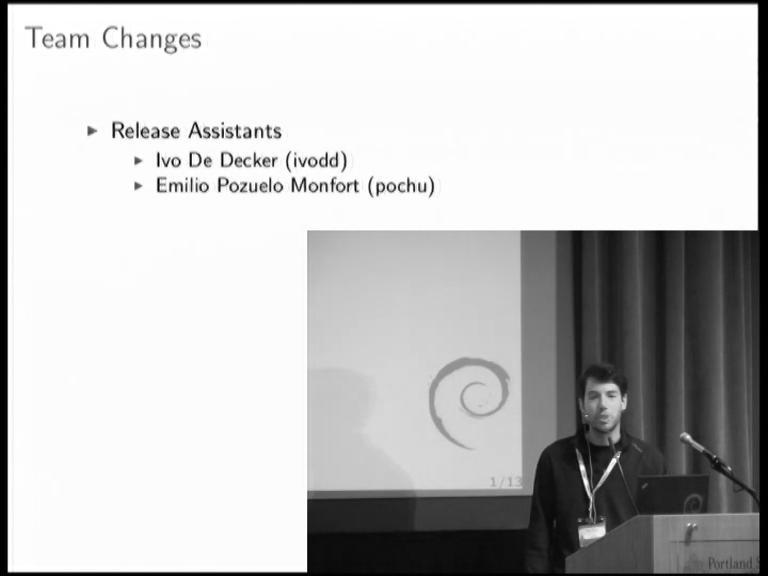
\includegraphics[width=5cm]{image201409/jessie_release_mono.png}
\end{wrapfigure}

 Releaseチームのセッションです。

 スライドは\url{https://release.debian.org/talks/debconf14/rt-debconf14.pdf}

 主な内容として、

\begin{itemize}
  \item freezeまでのタイムスケジュールと内容は以下の通り。
    \begin{itemize}
    \item 9/5に新規のtransitionを止める(ライブラリのアップグレードはここで終了)
    \item 10/5より緊急のアップロードを無視しはじめ、testingへの移行に10日かかるようになる。また、セキュリティチームからサポート不可のパッケージの吟味が行われるようになる。
    \item 11/5 Freezeする。
    \end{itemize}
\end{itemize}

\begin{itemize}
  \item 現在のRC bugの残りは450個。2/5以降、testingに移動するのが望ましくないと判断されたパッケージはremoveされる。基本的にどのパッケージもremoveから無事だとは思わないでほしいとのこと。
  \item 今から注意してほしい点として、今からはもう新規のtransitionを提案しないでほしい、Jessieに入れる気の無いパッケージのアップロードは一旦やめてほしい、とにかくインストールテスト(特にUEFI対応のPCを持っている人はできるだけ協力タノムとの事)と、バグを潰してほしいとのことです。
\end{itemize}

\subsection{日本の参加者の方の発表}

 今回、2名の日本からの参加者の方が発表をされていましたのでここに紹介しておきます。

\subsubsection{My PGPGPG key is RSA 2048bit but I put the private key on Gnuk Token}

\begin{wrapfigure}{r}{5cm}
  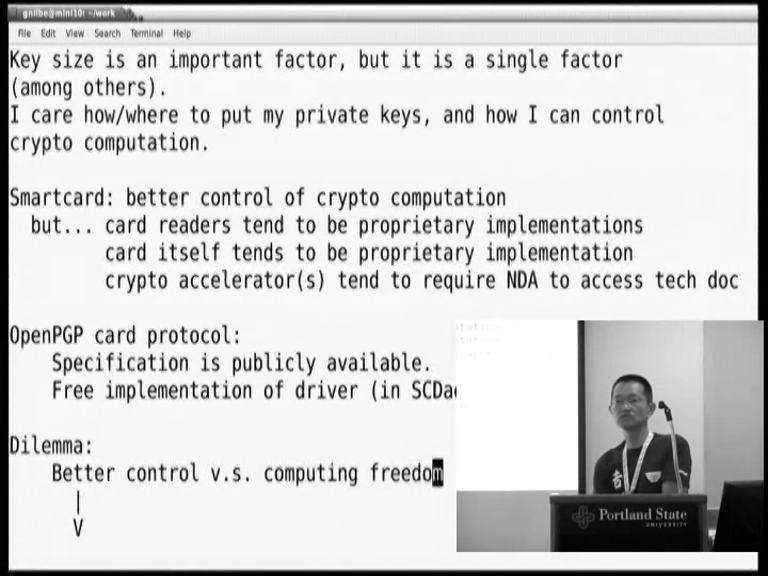
\includegraphics[width=5cm]{image201409/gnuk_mono.png}
\end{wrapfigure}

 新部さんのセッション。

 内容はGnuk Tokenの歴史と構造、動作の仕組みについてのセッションです。動作デモもありました。

 スライドは、\url{http://gobby.debian.org/export/debconf14/bof/gnuk}

 \begin{itemize}
  \item Gnuk Tokenは、gpgのセキュリティスマートデバイスとして動作できるUSBドングルの事。新部さん開発。このドングルを利用してgpgサインを行えば、暗号処理もドングル内部で行うため秘密鍵を不正に取り出されることもなくセキュアに署名・暗号化が出来る。    
 \end{itemize}

 \begin{itemize}
  \item Gnuk Tokenでは、乱数発生機として、未接続の内蔵ADコンバータの1ビット目を使ったとのこと。
  \item Gnuk Tokenは最大3つの鍵を扱えるとのこと。ストア可能なキーサイズは2kbytesはストアできる。
 \item 動作速度として、1.5秒でDebianパッケージのgpgサインが可能。
  \end{itemize}

 途中、ドングル売ってくれとの聴講者の要望があったのが印象的でした。

\subsubsection{find \& imporove some bottleneck in Debian project}

\begin{wrapfigure}{r}{5cm}
  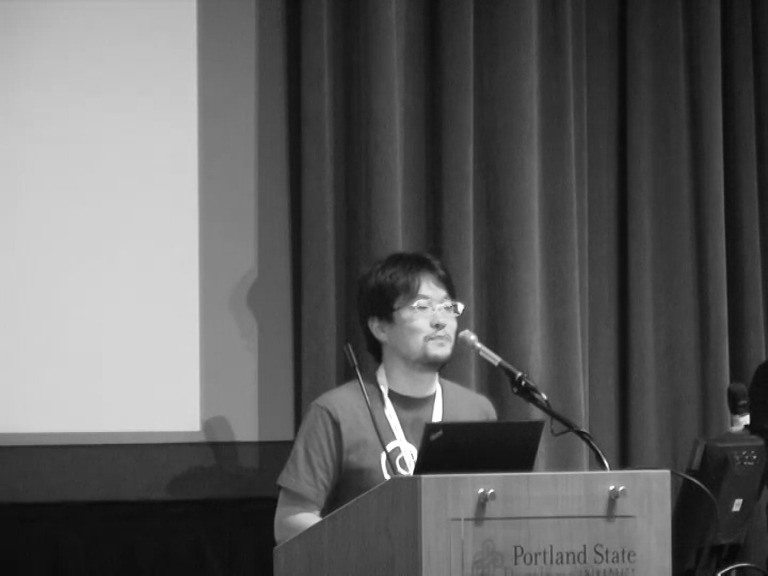
\includegraphics[width=5cm]{image201409/find_improve_mono.png}
\end{wrapfigure}

 やまねさんによるライトニングトーク(以下LT)中の発表。動画ファイル名Lightning\_Talks\_4.webm中 0:43:14あたりで発表。

 スライドは\url{http://www.slideshare.net/henrich_d/find-improve-some-bottleneck-in-debian-project-debconf14-lt}

 \begin{itemize}
  \item NEW キューのftpmasterによるチェックに時間がかかる事を解決したいという内容。現在ftpmasterだけが膨大な量のパッケージのレビュー作業・差し戻し作業をやっている事により、作業量が多すぎてNEW キューの受け入れが滞りがちという問題がある。
  \item ここでreview contributorという人を募集し、ftpmasterが現在行っているNEW キューのパッケージチェック作業を、彼ら(複数人)にやらせ、ftpmasterは最終の受け入れのOK/NGのみ出す役割にする。
 \end{itemize}

 \begin{itemize}
 \item review contributorは、Debian開発者候補としての訓練にも良いし、ftpmasterの作業が過多になってNEW キューが滞るのも解決できて一石二鳥でウマーというのがメリットなので、どうでしょう?という提案。
\end{itemize}

 こちらをきっかけに、Debian Projectに採用されると良いと思いました。

\subsection{その他}

 その他発表で興味深い内容のものを紹介します。

 \subsubsection{Debian in the Dark Ages of Free Software}

\begin{wrapfigure}{r}{5cm}
  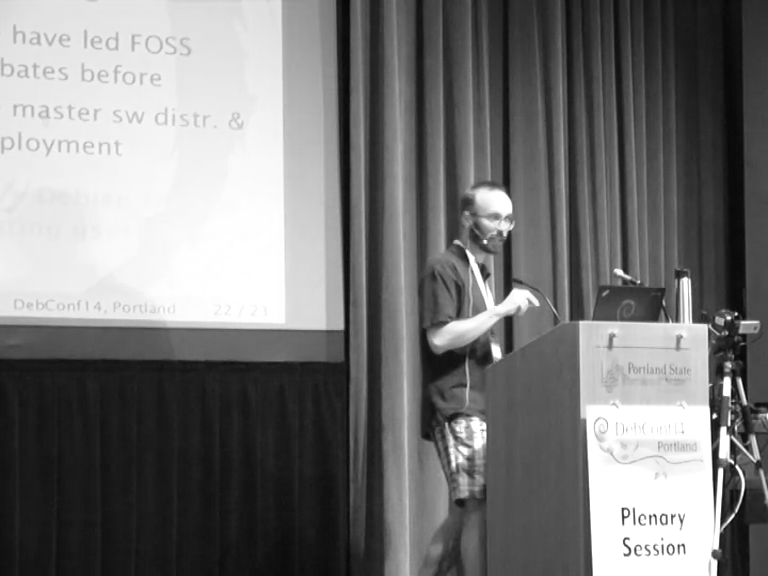
\includegraphics[width=5cm]{image201409/dark_age_mono.png}
\end{wrapfigure}

 2012年のDPLであったStefano Zacchiroli(以下zack)さんの発表です。

 \begin{itemize}
  \item DebianはDFSG Freeなdistoributionを作り普及させたことでは一定の成功を収めた。
 \item OSSも大変身近なものになり、ユーザは、たくさんのソフトウェアについて改変の自由が提供されるようになった。
  \item しかしながら、これらが成功した一方で、クラウドサービスも進化したため、せっかく勝ち取ったはずのソフトウェアの自由が、クラウドサービスの普及により、結局ユーザの手から取り上げられつつある。
 \item また、自由(Free)Softwareを作るにはFreeの開発ツール/開発環境が究極的には必須であるにもかかわらず、github/Gmailなどユーザからみれば自由でないサービスが益々開発ツール/環境としての地位を強固なものにしている。
 \end{itemize}

 \begin{itemize}
 \item このような時代にある事を認識し、これを自由(Free) Softwareの暗黒時代と呼ぼう。
\end{itemize}

 セッションでは、zackによるアイデアも披露され、また聴講者からも提案があったものの、zack曰くはっきりとした良い解決方法はまだ自分にもわからないという事でした。

 このセッションで示されている問題は、難しく由々しき問題です。共感される方は是非議論に提案に加わっていただけると幸いです。

\subsection{おわりに}

 他にもいろいろなセッションの動画が公開されています。ここでは紹介しきれなかったセッションにも面白いものが多数あります。

 興味がある方は是非視聴くださいませ。また、英語のヒアリングに自信のある方はDebConf Video subtitleチームに作業のご協力をおねがいします。

\begin{thebibliography}{9}
\bibitem{ref:osc-tokyo-2013-fall}OSC 2013 Tokyo/Fall 東京エリアDebian勉強会セミナ資料, \url{http://tokyodebian.alioth.debian.org/pdf/ debianmeetingresume201310-presentation.pdf}
\end{thebibliography}

%-------------------------------------------------------------------------------
\dancersection{Debian Trivia Quiz}{}
%-------------------------------------------------------------------------------

ところで、みなさん Debian 関連の話題においついていますか?Debian関連の話
題はメーリングリストをよんでいると追跡できます。ただよんでいるだけではは
りあいがないので、理解度のテストをします。特に一人だけでは意味がわからな
いところもあるかも知れません。みんなで一緒に読んでみましょう。

今回の出題範囲は\url{debian-devel-announce@lists.debian.org} や \url{debian-devel@lists.debian.org}に投稿された
内容とDebian Project Newsからです。

\begin{multicols}{2}
%; whizzy-master ../debianmeetingresume201311.tex
% 以上の設定をしているため、このファイルで M-x whizzytex すると、whizzytexが利用できます。
%

\santaku
{MATE desktop環境が先日Debianのパッケージに入りました。対象のMATEのバージョンは?}
{1.7}
{1.8}
{1.9}
{B}
{Gnome 2.28ベース以降のGnomeからフォークしたデスクトップ環境とのことです。読み方は「マテ」(マテ茶のマテ)と読むとのこと。}

\santaku
{ARM64アーキテクチャへの対応の協力者募集が行われました。残念ながらDebianは動きませんが、民生品で手に入るARM64搭載の機材は次のどれでしょう?}
{iphone 5s}
{NEXUS 7}
{OpenBlocks A7}
{A}
{iphone 5sから搭載されているA7 SoCはARMv8搭載でARM64動作も出来るそうです。ARM64を搭載した民生品はこれが最初かも。
一方、DebianのARM64ポーティングでは全く別の開発用向けに提供されている機材が利用されています。
我々がDebianの動くARM64機材を民生品で手に出来る日は何時ー(涙)?}

\santaku
{edos.debian.netがqa.debian.org/doseで復活しました。ところで、このサイト何するサイト?}
{各パッケージの依存関係がお互いに満たされている状態かをチェック}
{各パッケージがどれだけupstreamから乖離しているかチェック}
{各パッケージがどれだけ人気があるかをチェック}
{A}
{dose-*パッケージに含まれるチェックコマンドを使い、各アーキテクチャのdebianリポジトリを毎日チェックして、依存関係が満たされていないパッケージをチェックした結果を教えるサイトとなります。膨大な量のパッケージの依存関係を迅速にチェック出来るところが凄い点です。仕組みについてIEEEの論文まで出ているようです。参考:http://hal.archives-ouvertes.fr/ docs/00/14/95/66/PDF/ase.pdf}

\santaku
{先日Debian GNU/Hurdの中間報告がなされました。initが変更になったそうですが、どれになったでしょうか?}
{Hurd独自実装のinit}
{systemd}
{Sysvinit}
{C}
{去年のGSoCの成果がそのまま開発継続し、遂にSysvinitにinitが変更されたそうです。このおかげで、Network、halt/shutdown時の動作、ブート時のfilesystemのマウント方式がやっとDebian流になったようです。}

\santaku
{DEP-12がPTSによりサポートされたそうです。ところで、DEP-12の内容って何?}
{CIツールによる自動テストの為の定義ファイルの提案}
{upstreamに関する様々な情報を記載したメタデータの提案}
{copyrightファイルを機械処理がしやすいフォーマットにする提案}
{B}
{DEP-12はソースパッケージ中の''debian/upstream/metadata''等のファイルをに用意し、upstreamに関する様々な情報を記載しようという提案です。
 一方、「CIツールによる自動テストの為の...」はDEP-8であり、こちらは''debian/tests/''以下のファイルを使い、ci.debian.netでパッケージ開発について継続的インテグレーションを実施するものとなります。先日紹介のアナウンスありましたね。}

\santaku
{dputする前にはduckで必ずテストしてほしいとのこと。ところでduckって何?}
{debian/以下のファイルに含まれるURL/メールアドレスの存在をチェックするツール}
{状況・様子から名前を断定するツール}
{依存関係をチェックするツール}
{A}
{debian/controlファイル、debian/upstream関係のファイルに記載されているURL,メールアドレスのドメインパート(例:hoge@fuga.comのfuga.com部分)が実際に存在するか/アクセス可能かを調べてくれるツールがduckとなります。}

\santaku
{mentors.debian.netでレビュー待ちのパッケージはいくつある?}
{40〜50}
{50〜60}
{70以上}
{C}
{東京エリアDebian勉強会へいらっしゃるような皆様は、ぜひdebian-devel@debian.or.jpなどでDDにmentor役をお願いする、あるいはdebianの開発チームでパッケージがメンテナンスをされている場合はチームの誰かにmentor役をお願いするのがパッケージアップロードの道として早いです。不定期に開かれるDebian Hack Cafeで面前で直接頼むという手もあります。}

%; whizzy-master ../debianmeetingresume201311.tex
% 以上の設定をしているため、このファイルで M-x whizzytex すると、whizzytexが利用できます。
%

\santaku
{libcが変更になりました。変更前と変更後の組み合わせで正しいのはどれ?}
{eglibcからglibcへ変更}
{glibcからeglibcへ変更}
{uClibcからglibcへ変更}
{A}
{eglibcが採択されてから5年が経過し、glibcに戻ってきた状況です。}

\santaku
{ネットワークはTorを使い、ファイル/メール/メッセンジャーソフトは暗号化対応という特徴を持つdebianベースのLive OSの名前は何でしょう?}
{Plan9}
{Tails}
{GNU/Hurd}
{B}
{TrailsはThe Amnesic Incognito Live Systemの略です。利用者の出来る限りの匿名性を保つ事を目的として作られたDebianベースのlive osとなります。}

\santaku
{Debian 6 LTS開発の為の寄付を受け付ける会社名は?}
{Canonical}
{SquareEnix}
{Freexian}
{C}
{Freexian社は、Debianの公式開発者のRapha\"el Hertzogにより設立された、
Debianの有償サポートをするための会社です。}

\santaku
{jessieのデフォルトのgccのバージョンは何になった?}
{4.9}
{4.6}
{2.6}
{A}
{各パッケージはgcc-4.9でもコンパイルが通るように修正が必要となります。}

\santaku
{jessieのfreezeは11月5日です(注:リリースじゃないよ。)ここで、スケジュールで新規のtransitionが出来なくなる日はいつでしょう?}
{10月5日}
{9月5日}
{8月5日}
{B}
{9月5日以降は新規のtransitionが出来なくなります。新しいパッケージをjessieに合わせてリリースしようと目論む方々は期日にご注意下さい。}





%; whizzy-master ../debianmeetingresume201311.tex
% 以上の設定をしているため、このファイルで M-x whizzytex すると、whizzytexが利用できます。
%

\santaku
{2014/8/16にDebianは誕生日を迎えました。さて今年で何歳?}
{25}
{21}
{20}
{B}
{1993/8/16にIan Ashley Murdockさんにより、Debianは創設されました。というわけで、21歳です。Debian Dayはもう過ぎちゃいましたが、本日(2014/8/23)の勉強会後の宴会で祝いたいと思います!}

\santaku
{2014/7時点の各国のアクティブなDebian Developerの数とそれぞれの国の人口との比率が最も多いのはどこの国?}
{Finland}
{Ireland}
{New Zealand}
{A}
{Finlandは本割合は2009年からずっと毎年1位(今年3.61ppm。)2位 Ireland 3位 New Zealand。日本の本割合は0.28ppmで30位でした。単にアクティブDeveloperの絶対数が多い国は1位USA、2位Germany、3位France。}

\santaku
{OpenAmbitが2014/7にパッケージ化されsidへリリースされました。ところで何するパッケージ?}
{AmazonTV用アプリ開発環境}
{ChoromeCast用アプリ開発環境}
{SUNNTO AMBIT用アプリ開発環境}
{C}
{SUNNTO AMBITという腕時計型のGPS搭載の端末のアプリ開発環境となります。楽天とか、Amazonで買えます。スポーツ好きな方はDebianでアプリ開発やってみてください。}

\santaku
{2014/7/31にtechnical committeeによりDebianのデフォルトのJPEG圧縮伸長ライブラリとして採択されたのは以下のうちのどれ?}
{libjpeg6b}
{libjpeg8/9}
{libjpeg-turbo}
{C}
{libjpeg-turboはlibjpeg6 ABI互換のJPEG圧縮伸長ライブラリで、libjpeg6を遥かに凌ぐ速さで動作します。ここで、JPEG圧縮伸長ライブラリのデフォルトとして、libjpeg8/9か、libjpeg-turboかで議論が分かれていましたが、technical comitteeはlibjpeg-turboをデフォルトのJPEG圧縮伸長ライブラリとしました。}

\santaku
{2014/7/31にtechnical committeeから、「Debianパッケージは複数のinitシステムに対応する事」ということが再アナウンスされました。何のパッケージのドタバタがきっかけでしょう?}
{ftp}
{tftp-hpa}
{ncftp}
{B}
{experimentalにtftp-hpa 5.2-17が入ったが、そのchangelogとして''Removing upstart hacks, they are ugly and upstart is dead now.''という内容が入っていた件が物議を醸しました。bug746715参照。}

\santaku
{2014/7/20にsqueeze(注:squeeze-ltsではない)の最後のアップデートが行われました。何回目のアプデートでしょうか?}
{10}
{9}
{8}
{A}
{最後のsqueezeのアップデートです。実はこのアップデートを行っても、Debianですでに報告されているsqueezeのセキュリティホールの一部は残ったままです。しかしながら、これ以上のアップデートは無いので、wheezyにアップデートするか、squeeze-ltsの採用を検討しましょう。}

\santaku
{2014/7/31にJessieに搭載の可能性のあるlinux kernelのバージョンのアナウンスが行われました。バージョンはいくつでしょう?}
{3.14}
{3.12}
{3.16}
{C}
{2014/8/14にkernel.orgでlinux kernel3.16のリリースがアナウンスされました。Debian Kernelチームのアナウンスでは、「3.16がJessieに採用される可能性があるので、現在のパッケージが3.16と互換のあるKernel APIの元で動作するか確認し、問題があれば然るべき対応してほしい」とのこと。}

\santaku
{VCS-*フィールドのVCS情報を参照し、パッケージのchangelogが合致しているかのチェックが行われるようになりました。以下のどのサイトで確認できる?}
{http://qa.debian.org/cgi-bin/vcswatch}
{http://bugs.debian.org/}
{http://codesearch.debian.net/}
{A}
{vcswatchのページにアクセスし、見たいパッケージ名入れると、状況が得られます。詳しくはvcswatchのサイトの説明をご覧ください。}

\santaku
{パッケージに含まれているドキュメントに関して、lintianが新たな警告をするようになりました。以下のどれ?}
{HTMLファイル中の画像/CSS/JS/videoリンクがローカルファイルを指していない場合、警告}
{HTMLファイル中のDebianの綴りが間違っている場合、警告}
{HTMLファイルが入っていない場合、警告}
{A}
{ブラウザがHTMLファイルを表示する場合、ローカルのファイルであっても、表示時にブラウザが自動でリンク先をアクセスしてしまう作用を持つリンクがあります。ここに外部サイトのURLが入っていた場合、その外部サイトは、HTMLファイルが閲覧された時の情報を収集することが出来てしまいます。こういったことはセキュリティ上良くないので、該当するようなHTMLファイルが含まれている場合、lintianが警告するようになりました。}

\santaku
{2014/7にBTSのWEBサイトにreplyのリンクがつくようになりました。このリンクをブラウザからクリックすると何が起きるようになった?}
{BTS上でreplyしている次のメッセージが表示されるようになった。}
{BTS上のreply用のフォームがブラウザに表示されるようになった。}
{メーラが起動し、正しいSubject/宛先/引用が入るようになった。}
{C}
{やってみれば判りますが、Bugレポートに対する返答をする場合に、非常に便利です。BTSから見て、正しい内容と宛先で、返答出来るように下書きメールがメーラに準備されるようになりました。}

\santaku
{2014/8/14にDebian Installer Jessie Beta 1がアナウンスされました。このバージョンのインストーラで導入されるinitシステムは結局どうなった?}
{systemdになった}
{sysvinitになった}
{upstartになった}
{A}
{このバージョンのDebian Installerから、initシステムとしてsystemdが入るようになりました。ちなみにこの件、Installerプログラム本体の話であって、Jessie本体のBeta版リリースという意味では無い事に注意。}

%; whizzy-master ../debianmeetingresume201311.tex
% 以上の設定をしているため、このファイルで M-x whizzytex すると、whizzytexが利用できます。
%

\santaku
{FSFがDebian Projectへ案内をしてきた、自由ソフトウェアのみの元で動かすことの出来るハードウェアについてのデータベースは次のうちどれ?}
{h-node.org}
{wiki.debian.org/Hardware}
{openbenchmarking.org}
{A}
{日本語の本件のニュースはsourceforge.jpの記事参照:http://sourceforge.jp/magazine/14/09/11/062900 。FSFはmainリポジトリのみのパッケージで構成されるDebianは自由ソフトウェアとみているとのこと。}

\santaku
{Debconf14の参加人数は結局何人?}
{900人}
{300人}
{1000人}
{B}
{300人とのことです。参考:Debconf13は290人、Debconf12は176人、Debconf11は335人でした。}

\santaku
{8/17にbuilddにて使われるアーカイブがどこからもアクセスできるようになりました。urlはどれ?}
{ftp.debian.or.jp/debian/}
{ftp.jp.debian.org/debian/}
{incoming.debian.org/debian-buildd/}
{C}
{今までは、どこからもアクセスできたわけではなかったようです。}

\santaku
{2014/8/19に登録商標としてDebianロゴが正式に登録されたそうです。どこの国の登録商標でしょうか?}
{米国}
{日本}
{スイス}
{A}
{United States Patent and Trademark Officeになります(つまり米国。)登録されたDebianロゴのデザインは http://tdr.uspto.gov/search.action?sn=86037470 からたどると閲覧できます。}

\santaku
{2014/8/24のBitFromDPLによれば、Debian Projectは仮想通貨による寄付をはじめて受け付けたそうです。具体的には何という仮想通貨でしょう?}
{Greeコイン}
{Crysta}
{BitCoin}
{C}
{Debian ProjectはBitCoinをそのまま受け付けることが出来るシステムを持たないため、その場限りの方法で受け取ったとのことです。今後、こういった仮想通貨での寄付の受け取りと取り扱いについて意見がほしいとのことです。}

\santaku
{検索エンジンのDuckDuckGOより、収入が入ったとのことです。2014/8/24現在、月当たりのDuckDuckGOからの平均収入は月額いくらでしょう?}
{\$10}
{\$152}
{\$1400}
{B}
{Debianパッケージに含まれるブラウザにデフォルトで登録されている検索エンジンの候補としてDuckDuckGOが搭載されていることによる収入となります。DuckDuckGOはプライバシーに配慮した検索エンジンです。最近は、iphone のsafariブラウザにあらかじめ登録される検索エンジンの候補としても上がり有名になりつつあります。URLはhttps://duckduckgo.com/}

\santaku
{2014/8/27にDebian archiveに搭載された2つの新しいアーキテクチャは、arm64以外には以下のどれ?}
{sparc}
{mips}
{ppc64el}
{C}
{ 64 bit powerpcのlittle endianモードのポーティングとのことです。すでに存在するppc64はbig endianのバイナリのポートティングとなります。}

\santaku
{2014/8/31にて、arm64ポートのDebian開発用に、無償のARM64用のコンパイラ・デバッガ等の開発キットの提供が行われたようです。製品名は以下のどれ?}
{Microsoft Visual Studio}
{IAR Embedded Workbench}
{DS-5 Development Studio}
{C}
{ Debian Editionとのことです。アナウンスによれば、ダウンロードリンクは http://ds.arm.com/debian/ からダウンロード可能とのことですが、日本からはダウンロードが現在出来ない模様です。残念!もちろんですが、この開発キットは無償ではあるものの自由ソフトウェアではないので誤解なきよう。}

\santaku
{ Debian keyringからある大きさ以上の秘密鍵長を持たないキーが2014/12/31以降で削除される事についてのリマインドのアナウンスが流れていました。ある大きさとは以下のどれ?}
{ 512bit }
{ 2048bit }
{ 4096bit }
{B}
{ キーサインにつかうgpgの鍵も2048bit以上にしましょう!}

\santaku
{ 2014/9/17にDebian Policy が改定されました。改定後のバージョンはいくつ?}
{ 3.9.5.0 }
{ 3.9.6.0 }
{ 4.0.0.0 }
{B}
{ パッケージ開発をする前に、新しいDebian Policyの変更差分は読んでおきましょう。}

%; whizzy-master ../debianmeetingresume201311.tex
% 以上の設定をしているため、このファイルで M-x whizzytex すると、whizzytexが利用できます。
%

\santaku
{2014/9/14時点でJessieでサポートされると残念ながら「言われなかった」アーキテクチャはどれ}
{amd64}
{powerpc}
{sparc}
{C}
{2014/9/14時点でサポートされると言われたアーキテクチャは:amd64,armel,armhf,i386,kfreebsd-amd64/kfreebsd-i386/mips/mipsel/powerpc/s390x。なお、arm64/ppc64elは好調な頑張りとのことで、この調子が続けば入るかも??という状況。}

\santaku
{2014/11/1時点でJessieでサポートされるかどうかについて依然として懸念のあるものはどれ}
{hurd}
{kFreeBSD}
{s390x}
{B}
{kFreeBSDは頑張って欲しいとのこと。最終ジャッジは2014/11/1に行われる。なお、s390xは9/14では懸念なし、hurdはすでにリリースは無理との判断になっている。}

\santaku
{2014/9/4にtesting入りしたデスクトップ環境は以下のどれ}
{xfce}
{cinnamon}
{unity}
{B}
{cinnamonはGTK+3を利用して作られたデスクトップ環境です。元々はLinux MINT向けにGNOME Shellからforkしたデスクトップシェルでした。開発が続き、デスクトップシェルから発展して遂にデスクトップ環境となりました。}

\santaku
{2014/10/18にリリースされたwheezyのDebianのバージョンはいくら?}
{7.7}
{7.8}
{7.9}
{A}
{7回目のアップデートとなります。早速アップグレードしましょう!新規にインストールする安定版ならDebian7.7からやりましょう!}

\santaku
{OPWの呼びかけがdebian-devel-announceで2014/9/30に行われました。ところでOPWって何の略?}
{One-time PassWord}
{One-Piece-Woven technology}
{Outreach-Program-for-Women}
{C}
{Outreach-Program-for-Women(略してOPW)は、GNOME Foundationが始めた、FOSSのプロジェクトの貢献者にもっと女性を増やそう!という活動となります。FOSSの貢献者の男女構成比は、圧倒的に男の割合が高いといういびつな傾向があるため、こちらを是正しようとする活動です。}

\santaku
{2014/10/14にサービスを近いうちに閉じるよとアナウンスのあったサイトはどれでしょう?}
{githubredir.debian.net}
{tracker.debian.org}
{rtc.debian.org}
{A}
{githubredir.debian.netは、github上にあるupstreamのソースについて、リリースの為にバージョン番号でtag打ちされたバージョンのソースのtarボールに対する直接のリンクを統一的な書式のURLで生成するサービスです。つまり、debian/watchにupstreamのソースの有りかを書きやすくするために使われます。githubが改善され今となっては不要となってしまったということもあり、近いうちに廃止するというアナウンスが行われました。}

\santaku
{2014/10/5にリリースされたDebian Installer Jessie Beta2の変更点はどれ}
{syslinuxまわりで過去の互換の無い大きな変更点が出た。}
{デフォルトのinitがsystemdとなった。}
{GNOMEデスクトップ環境がデフォルトになった。}
{C}
{一度はXfceデスクトップ環境と言われていましたが、accessibilityの完成度の高さには勝てず、再びGNOMEに戻ってきた形となりました。なお、他の選択肢はBeta1の時の変更点となります。}

\santaku
{2014/10/16に投票が開始されました。内容は次のうちどれ?}
{特定のinitとプログラムが依存しても良いか?ダメか?程度次第か?}
{GNOMEをデフォルトにしてよいのか?}
{野島が勉強会幹事をやり続けて良いのか?}
{A}
{Debianの各種initシステムと他アプリケーションの依存についての規定に関する投票となります。投票内容について詳しくはhttps://www.debian.org/vote/2014/vote\_003。ところで、Debianのイベントの幹事は、もちろん、いつ、誰が、どのようにやってもよくてよ?勇者の数を増やせ!}

%; whizzy-master ../debianmeetingresume201311.tex
% 以上の設定をしているため、このファイルで M-x whizzytex すると、whizzytexが利用できます。
%

\santaku
{Debian Project関係者のPodCastのサイトが公開されました。以下のどれ?}
{www.debian.org}
{www.debianandstuff.com}
{www.debian.or.jp}
{B}
{英語です。記念すべき第1回目は「MoinMoin Vs. MediaWiki」であり、パーソナリティーはAsheesh Laroiaさんと、Sam Erbsさんとなります。収録はDebConf14中に収録したそうです。}

\santaku
{2014/10/27のDPNにAda initiativeから寄付のアナウンスの件が載っていました。Ada initiativeって何?}
{オープンなテクノロジに関して女性活躍の支援をする団体}
{プログラミング言語Adaの普及促進をする団体}
{Adaさんの政治後援会}
{A}
{オープンなテクノロジに関して女性活躍の支援が活発になってきました。Debianでは、Debian Womenというプロジェクトがあります。Gnome Foundationが2006年にFree \& Open Source Software Outreach Program(略してOPW)を開始したのがきっかけで、Debian Projectもこちらの動きに賛同している状況です。}

\santaku
{2014/10/27にDebianのwhoisコマンドが入れ替わりました。特徴はどれ?}
{サイズが小さくなった}
{DFSGに準拠した}
{作者独自の調査によりIANAの情報より正確になった}
{C}
{今までBSD由来のwhoisコマンドがDebianで使われてきましたが、この度Marcoさん作のwhoisコマンドに変わりました。Marcoさんは1年を費やして、IANAよりも正確に情報を得られるサーバ群を独自の調査で探し当て、こちらで対応するようにしたそうです。なお、Marcoさんのwhoisコマンドは全Linuxディストリビューションの標準のwhoisコマンドになるそうです。}

\santaku
{2014/10/15時点で、Freexianと契約したDebianのLTSのスポンサーは全部で何社?}
{14社}
{13社}
{12社}
{A}
{\url{http://raphaelhertzog.com/2014/10/15/freexians-second-report-about-debian-long-term-support/}に掲載されています。こちらのスポンサーのお陰で、LTSを担当できるDebian開発者らのフルタイムのうち、25\%の時間を割く事ができるようになったとのことです。古いDebianを使っている会社さんは是非スポンサーになってくださいませ。}

\santaku
{2014/10/27のDPNにてDebian Multimediaの進捗状況報告がありました。libav6:11で搭載された新しい機能は次のうちどれ。}
{libx265-encoder}
{libx265-decoder}
{libx264-encoder}
{A}
{libav6:11はjessie搭載予定のMultimedia用codecライブラリです。遂にx265のエンコーダが搭載されたようです。x265は、ワンセグなどで使われている高性能なコーデックのH.264/MPEG-4 AVCの後継であるH.265の互換実装となります。H.265はH.264の2倍の圧縮率を誇るとのことで、Jessieでの動画鑑賞が楽しみですね。}

\santaku
{2014/11/5にてFreezeが行われました。この時残っているRC bugは何個だったでしょう?}
{200個}
{310個}
{400個}
{B}
{Freeze時に310個しかRC bugがなかったのは、昨今のFreezeではなかったほどの快挙だそうです。さあ、RC bug潰しまくりましょう!}

\santaku
{2014/10/27にて初めてJessieベースのDebianEduがリリースされました。DebianEduはDebianの用語ではどのしくみに分類されるでしょうか?}
{Derivative}
{Blend}
{PureBlend}
{C}
{PureBlendは、特定用途向けのDebianに仕上がるようにインストールを行う場合、controlファイルに必要なパッケージをRecommendsで指定しただけのパッケージを用意することによって、簡単にDebianパッケージ群のみをまとめてインストールできるようにするためのしくみです。詳しくは、「第108回東京エリアDebian勉強会、2014年1月勉強会」(http://tokyodebian.alioth.debian.org/2014-01.html)の資料に詳しいです。}

\santaku
{Jessieから取り除かれる予定のQtのバージョンはいくつでしょう?}
{Qt3}
{Qt4}
{Qt5}
{B}
{Qt4はupstream側で2015年に開発を終了する決定となりました。Jessieに搭載予定のQtのバージョンはQt5となります。}

\santaku
{mainパッケージのDependsフィールドに''package-in-main | packages-non-free''と書いて良いかどうかの決定が2014/10/31にTechnicalCommiteeにより下されました。結論は以下のうちのどれ?}
{状況次第でOKだったり、NGだったり}
{NG}
{OK}
{C}
{例えば、''Depends: unrar-free | rar''というようなパターンがありえます。通常は、mainパッケージで構成されるDebianシステムはDFSG準拠であるべきなので、「non-freeパッケージのみ」に依存するようなパッケージをmain側に作ってはいけないというルールがあります。今回の場合は、mainパッケージのリポジトリ指定時に、non-freeのパッケージが優先して導入されることは無いのでOKとなりました。}

\santaku
{2014/11/9のRelease TeamからDebian 9,Debian 10のコードネームが決まりました。Debian 10のコードネームは次のうちのどれ?}
{Buster}
{Stretch}
{Jessie}
{A}
{ちなみにDebian 9は''Strech''だそうです。}

\santaku
{2014/11/9のRelease Teamのメールにて、arm64, ppc64el, kfreebsdについて、Jessieの公式リリースに含むかどうかの決断が行われました。「含まない」とされたのは次のうちどれ?}
{arm64}
{ppc64el}
{kfreebsd}
{C}
{大変遺憾ながら、kfreebsdは、期日までにJessie公式リリースに必要とされる品質に達しなかったとの事です。ただ、kfreebsdがDebianプロジェクト自体から消えるわけではないので、Jessie公式リリース時期に、条件が揃えば非公式のリリースとして扱う事が可能とのことです。このパターンになったのは、Debian GNU/Hurd 2013が2013年にそのようなリリースを行ったことがあります。}

\santaku
{2014/11/14にて、Debian Medチームから、とあるパッケージをやっとDFSG準拠にすることが出来たとの報告がありました。そのパッケージ名は以下のどれ?}
{abyss}
{arb}
{phylip}
{C}
{upstreamはワシントン大学であるphylipは、bioinfomaticsでは有名なソフトウェアとのことです。しかしながら、ワシントン大学の課しているライセンスは、非営利の研究用途のみに利用を許諾している状態でした。こちらについて長年のDebian Medの交渉により、遂にphylipはDFSG準拠の自由ライセンスにしてもらえたとのことです。また、phylipが原因でnon-freeにせざるを得なかったseaviewというパッケージも無事mainにすることが出来るとのことでした。}

\end{multicols}

%for less page
%\printindex

% 問題と回答が同じみひらきにならないようにする
\cleartooddpage
%-------------------------------------------------------------------------------
\dancersection{Debian Trivia Quiz 問題回答}{}
%-------------------------------------------------------------------------------

 Debian Trivia Quiz の問題回答です。
 あなたは何問わかりましたか? \\
 %回答はdebianmeetingresume2014-fuyu.jqzというファイルに生成されるので、
 %それを手動でコピペして使う。
 % ここからコピペ
 % FIXME 問題が全部はいったらコピペすること
 %(progn (next-line 1)(insert-file "debianmeetingresume2013-fuyu.jqz") )
 \begin{itemize}
 \item
1. B Gnome 2.28ベース以降のGnomeからフォークしたデスクトップ環境とのことです。読み方は「マテ」(マテ茶のマテ)と読むとのこと。
\item
2. A iphone 5sから搭載されているA7 SoCはARMv8搭載でARM64動作も出来るそうです。ARM64を搭載した民生品はこれが最初かも。一方、DebianのARM64ポーティングでは全く別の開発用向けに提供されている機材が利用されています。我々がDebianの動くARM64機材を民生品で手に出来る日は何時ー(涙)?
\item
3. A dose-*パッケージに含まれるチェックコマンドを使い、各アーキテクチャのdebianリポジトリを毎日チェックして、依存関係が満たされていないパッケージをチェックした結果を教えるサイトとなります。膨大な量のパッケージの依存関係を迅速にチェック出来るところが凄い点です。仕組みについてIEEEの論文まで出ているようです。参考:http://hal.archives-ouvertes.fr/ docs/00/14/95/66/PDF/ase.pdf
\item
4. C 去年のGSoCの成果がそのまま開発継続し、遂にSysvinitにinitが変更されたそうです。このおかげで、Network、halt/shutdown時の動作、ブート時のfilesystemのマウント方式がやっとDebian流になったようです。
\item
5. B DEP-12はソースパッケージ中の''debian/upstream/metadata''等のファイルをに用意し、upstreamに関する様々な情報を記載しようという提案です。一方、「CIツールによる自動テストの為の...」はDEP-8であり、こちらは''debian/tests/''以下のファイルを使い、ci.debian.netでパッケージ開発について継続的インテグレーションを実施するものとなります。先日紹介のアナウンスありましたね。
\item
6. A debian/controlファイル、debian/upstream関係のファイルに記載されているURL,メールアドレスのドメインパート(例:hoge@fuga.comのfuga.com部分)が実際に存在するか/アクセス可能かを調べてくれるツールがduckとなります。
\item
7. C 東京エリアDebian勉強会へいらっしゃるような皆様は、ぜひdebian-devel@debian.or.jpなどでDDにmentor役をお願いする、あるいはdebianの開発チームでパッケージがメンテナンスをされている場合はチームの誰かにmentor役をお願いするのがパッケージアップロードの道として早いです。不定期に開かれるDebian Hack Cafeで面前で直接頼むという手もあります。
\item
8. A eglibcが採択されてから5年が経過し、glibcに戻ってきた状況です。
\item
9. B TrailsはThe Amnesic Incognito Live Systemの略です。利用者の出来る限りの匿名性を保つ事を目的として作られたDebianベースのlive osとなります。
\item
10. C Freexian社は、Debianの公式開発者のRapha\"el Hertzogにより設立された、Debianの有償サポートをするための会社です。
\item
11. A 各パッケージはgcc-4.9でもコンパイルが通るように修正が必要となります。
\item
12. B 9月5日以降は新規のtransitionが出来なくなります。新しいパッケージをjessieに合わせてリリースしようと目論む方々は期日にご注意下さい。
\item
13. B 1993/8/16にIan Ashley Murdockさんにより、Debianは創設されました。というわけで、21歳です。Debian Dayはもう過ぎちゃいましたが、本日(2014/8/23)の勉強会後の宴会で祝いたいと思います!
\item
14. A Finlandは本割合は2009年からずっと毎年1位(今年3.61ppm。)2位 Ireland 3位 New Zealand。日本の本割合は0.28ppmで30位でした。単にアクティブDeveloperの絶対数が多い国は1位USA、2位Germany、3位France。
\item
15. C SUNNTO AMBITという腕時計型のGPS搭載の端末のアプリ開発環境となります。楽天とか、Amazonで買えます。スポーツ好きな方はDebianでアプリ開発やってみてください。
\item
16. C libjpeg-turboはlibjpeg6 ABI互換のJPEG圧縮伸長ライブラリで、libjpeg6を遥かに凌ぐ速さで動作します。ここで、JPEG圧縮伸長ライブラリのデフォルトとして、libjpeg8/9か、libjpeg-turboかで議論が分かれていましたが、technical comitteeはlibjpeg-turboをデフォルトのJPEG圧縮伸長ライブラリとしました。
\item
17. B experimentalにtftp-hpa 5.2-17が入ったが、そのchangelogとして''Removing upstart hacks, they are ugly and upstart is dead now.''という内容が入っていた件が物議を醸しました。bug746715参照。
\item
18. A 最後のsqueezeのアップデートです。実はこのアップデートを行っても、Debianですでに報告されているsqueezeのセキュリティホールの一部は残ったままです。しかしながら、これ以上のアップデートは無いので、wheezyにアップデートするか、squeeze-ltsの採用を検討しましょう。
\item
19. C 2014/8/14にkernel.orgでlinux kernel3.16のリリースがアナウンスされました。Debian Kernelチームのアナウンスでは、「3.16がJessieに採用される可能性があるので、現在のパッケージが3.16と互換のあるKernel APIの元で動作するか確認し、問題があれば然るべき対応してほしい」とのこと。
\item
20. A vcswatchのページにアクセスし、見たいパッケージ名入れると、状況が得られます。詳しくはvcswatchのサイトの説明をご覧ください。
\item
21. A ブラウザがHTMLファイルを表示する場合、ローカルのファイルであっても、表示時にブラウザが自動でリンク先をアクセスしてしまう作用を持つリンクがあります。ここに外部サイトのURLが入っていた場合、その外部サイトは、HTMLファイルが閲覧された時の情報を収集することが出来てしまいます。こういったことはセキュリティ上良くないので、該当するようなHTMLファイルが含まれている場合、lintianが警告するようになりました。
\item
22. C やってみれば判りますが、Bugレポートに対する返答をする場合に、非常に便利です。BTSから見て、正しい内容と宛先で、返答出来るように下書きメールがメーラに準備されるようになりました。
\item
23. A このバージョンのDebian Installerから、initシステムとしてsystemdが入るようになりました。ちなみにこの件、Installerプログラム本体の話であって、Jessie本体のBeta版リリースという意味では無い事に注意。
\item
24. A 日本語の本件のニュースはsourceforge.jpの記事参照:http://sourceforge.jp/magazine/14/09/11/062900 。FSFはmainリポジトリのみのパッケージで構成されるDebianは自由ソフトウェアとみているとのこと。
\item
25. B 300人とのことです。参考:Debconf13は290人、Debconf12は176人、Debconf11は335人でした。
\item
26. C 今までは、どこからもアクセスできたわけではなかったようです。
\item
27. A United States Patent and Trademark Officeになります(つまり米国。)登録されたDebianロゴのデザインは http://tdr.uspto.gov/search.action?sn=86037470 からたどると閲覧できます。
\item
28. C Debian ProjectはBitCoinをそのまま受け付けることが出来るシステムを持たないため、その場限りの方法で受け取ったとのことです。今後、こういった仮想通貨での寄付の受け取りと取り扱いについて意見がほしいとのことです。
\item
29. B Debianパッケージに含まれるブラウザにデフォルトで登録されている検索エンジンの候補としてDuckDuckGOが搭載されていることによる収入となります。DuckDuckGOはプライバシーに配慮した検索エンジンです。最近は、iphone のsafariブラウザにあらかじめ登録される検索エンジンの候補としても上がり有名になりつつあります。URLはhttps://duckduckgo.com/
\item
30. C 64 bit powerpcのlittle endianモードのポーティングとのことです。すでに存在するppc64はbig endianのバイナリのポートティングとなります。
\item
31. C Debian Editionとのことです。アナウンスによれば、ダウンロードリンクは http://ds.arm.com/debian/ からダウンロード可能とのことですが、日本からはダウンロードが現在出来ない模様です。残念!もちろんですが、この開発キットは無償ではあるものの自由ソフトウェアではないので誤解なきよう。
\item
32. B キーサインにつかうgpgの鍵も2048bit以上にしましょう!
\item
33. B パッケージ開発をする前に、新しいDebian Policyの変更差分は読んでおきましょう。
\item
34. C 2014/9/14時点でサポートされると言われたアーキテクチャは:amd64,armel,armhf,i386,kfreebsd-amd64/kfreebsd-i386/mips/mipsel/powerpc/s390x。なお、arm64/ppc64elは好調な頑張りとのことで、この調子が続けば入るかも??という状況。
\item
35. B kFreeBSDは頑張って欲しいとのこと。最終ジャッジは2014/11/1に行われる。なお、s390xは9/14では懸念なし、hurdはすでにリリースは無理との判断になっている。
\item
36. B kFreeBSDは頑張って欲しいとのこと。最終ジャッジは2014/11/1に行われる。なお、s390xは9/14では懸念なし、hurdはすでにリリースは無理との判断になっている。
\item
37. B cinnamonはGTK+3を利用して作られたデスクトップ環境です。元々はLinux MINT向けにGNOME Shellからforkしたデスクトップシェルでした。開発が続き、デスクトップシェルから発展して遂にデスクトップ環境となりました。
\item
38. A 7回目のアップデートとなります。早速アップグレードしましょう!新規にインストールする安定版ならDebian7.7からやりましょう!
\item
39. C Outreach-Program-for-Women(略してOPW)は、GNOME Foundationが始めた、FOSSのプロジェクトの貢献者にもっと女性を増やそう!という活動となります。FOSSの貢献者の男女構成比は、圧倒的に男の割合が高いといういびつな傾向があるため、こちらを是正しようとする活動です。
\item
40. A githubredir.debian.netは、github上にあるupstreamのソースについて、リリースの為にバージョン番号でtag打ちされたバージョンのソースのtarボールに対する直接のリンクを統一的な書式のURLで生成するサービスです。つまり、debian/watchにupstreamのソースの有りかを書きやすくするために使われます。githubが改善され今となっては不要となってしまったということもあり、近いうちに廃止するというアナウンスが行われました。
\item
41. C 一度はXfceデスクトップ環境と言われていましたが、accessibilityの完成度の高さには勝てず、再びGNOMEに戻ってきた形となりました。なお、他の選択肢はBeta1の時の変更点となります。
\item
42. A Debianの各種initシステムと他アプリケーションの依存についての規定に関する投票となります。投票内容について詳しくはhttps://www.debian.org/vote/2014/vote\_003。ところで、Debianのイベントの幹事は、もちろん、いつ、誰が、どのようにやってもよくてよ?勇者の数を増やせ!
\item
43. B 英語です。記念すべき第1回目は「MoinMoin Vs. MediaWiki」であり、パーソナリティーはAsheesh Laroiaさんと、Sam Erbsさんとなります。収録はDebConf14中に収録したそうです。
\item
44. A オープンなテクノロジに関して女性活躍の支援が活発になってきました。Debianでは、Debian Womenというプロジェクトがあります。Gnome Foundationが2006年にFree \& Open Source Software Outreach Program(略してOPW)を開始したのがきっかけで、Debian Projectもこちらの動きに賛同している状況です。
\item
45. C 今までBSD由来のwhoisコマンドがDebianで使われてきましたが、この度Marcoさん作のwhoisコマンドに変わりました。Marcoさんは1年を費やして、IANAよりも正確に情報を得られるサーバ群を独自の調査で探し当て、こちらで対応するようにしたそうです。なお、Marcoさんのwhoisコマンドは全Linuxディストリビューションの標準のwhoisコマンドになるそうです。
\item
46. A {\footnotesize{\url{http://raphaelhertzog.com/2014/10/15/freexians-second-report-about-debian-long-term-support/}}}に掲載されています。こちらのスポンサーのお陰で、LTSを担当できるDebian開発者らのフルタイムのうち、25\%の時間を割く事ができるようになったとのことです。古いDebianを使っている会社さんは是非スポンサーになってくださいませ。
\item
47. A libav6:11はjessie搭載予定のMultimedia用codecライブラリです。遂にx265のエンコーダが搭載されたようです。x265は、ワンセグなどで使われている高性能なコーデックのH.264/MPEG-4 AVCの後継であるH.265の互換実装となります。H.265はH.264の2倍の圧縮率を誇るとのことで、Jessieでの動画鑑賞が楽しみですね。
\item
48. B Freeze時に310個しかRC bugがなかったのは、昨今のFreezeではなかったほどの快挙だそうです。さあ、RC bug潰しまくりましょう!
\item
49. C PureBlendは、特定用途向けのDebianに仕上がるようにインストールを行う場合、controlファイルに必要なパッケージをRecommendsで指定しただけのパッケージを用意することによって、簡単にDebianパッケージ群のみをまとめてインストールできるようにするためのしくみです。詳しくは、「第108回東京エリアDebian勉強会、2014年1月勉強会」(http://tokyodebian.alioth.debian.org/2014-01.html)の資料に詳しいです。
\item
50. B Qt4はupstream側で2015年に開発を終了する決定となりました。Jessieに搭載予定のQtのバージョンはQt5となります。
\item
51. C 例えば、''Depends: unrar-free | rar''というようなパターンがありえます。通常は、mainパッケージで構成されるDebianシステムはDFSG準拠であるべきなので、「non-freeパッケージのみ」に依存するようなパッケージをmain側に作ってはいけないというルールがあります。今回の場合は、mainパッケージのリポジトリ指定時に、non-freeのパッケージが優先して導入されることは無いのでOKとなりました。
\item
52. A ちなみにDebian 9は''Strech''だそうです。
\item
53. C 大変遺憾ながら、kfreebsdは、期日までにJessie公式リリースに必要とされる品質に達しなかったとの事です。ただ、kfreebsdがDebianプロジェクト自体から消えるわけではないので、Jessie公式リリース時期に、条件が揃えば非公式のリリースとして扱う事が可能とのことです。このパターンになったのは、Debian GNU/Hurd 2013が2013年にそのようなリリースを行ったことがあります。
\item
54. C upstreamはワシントン大学であるphylipは、bioinfomaticsでは有名なソフトウェアとのことです。しかしながら、ワシントン大学の課しているライセンスは、非営利の研究用途のみに利用を許諾している状態でした。こちらについて長年のDebian Medの交渉により、遂にphylipはDFSG準拠の自由ライセンスにしてもらえたとのことです。また、phylipが原因でnon-freeにせざるを得なかったseaviewというパッケージも無事mainにすることが出来るとのことでした。
\end{itemize}

% add page to even number
\newpage
\thispagestyle{empty}\mbox{}

\newpage
%\thispagestyle{empty}\mbox{}
%\newpage

\thispagestyle{empty}
{
\large
\begin{itembox}{\bf 『あんどきゅめんてっど でびあん』について}
本書は、東京および関西周辺で毎月行なわれている『東京エリア Debian 勉強会』および
『関西 Debian 勉強会』で
使用された資料・小ネタ・必殺技などを一冊にまとめたものです。
% FIXME: 範囲を修正すること。
収録範囲は2014/06〜2014/11まで
東京エリアは第114回から第120回までおよび、
関西エリアは第85回から第91回まで(第 86 回関西 Debian 勉強会 は OSC2014 Kansai@Kyotoのため無し
第87-89回はもくもく会のため収録無し、第 90 回 関西 Debian 勉強会 は 関西オープンフォーラム 2014、
第 91 回 関西 Debian 勉強会 Jessieインストーラテスト会のためなし)。
内容は無保証、つっこみなどがあれば勉強会にて。
\end{itembox}
}

\vspace*{13cm}
{\color{dancerlightblue}\rule{\hsize}{1mm}}
\vspace{2mm}

\includegraphics[width=2cm]{image200502/openlogo-nd.eps}
\noindent \Large \bf あんどきゅめんてっど でびあん 2014年冬号\\
\noindent \normalfont 2014年12月30日 \hspace{5mm}  初版第1刷発行\\
\noindent \normalfont 東京エリア Debian 勉強会/関西Debian 勉強会 (編集・印刷・発行)\\
{\color{dancerdarkblue}\rule{\hsize}{1mm}}

\end{document}
